\documentclass[11pt,letterpaper]{article}
\input{headings}
\usepackage{soul}
\newcommand \recipeName {Daniel's Chocolate Mousse}
\newcommand \fileName {ChocolateMousse}
\chead{\recipeName}

\begin{document}
\input{title}


This is a dairy-free Chocolate Mousse. The base for this recipe is the cream that I learned to make from Bebe Brown, Scott's grandmother, in her kitchen in Oklahoma in the 1990s. She always made perfect cream pies. In one of the Christmas holidays I stood behind her and took notes as she prepared a pie from memory. 
	
\begin{description}
\item[Ingredients:]\ \\
	\begin{itemize}
	\item 3 cups of almond milk (25 1/2 oz = 1 pound + 9 1/2 oz = 722 grams)
	\item 1 cup of sugar (7 oz = 200 grams)
	\item 2 Tablespoon of corn starch (1/2 oz = 15 grams)
	\item 1/4 cup of flour (1 1/4 oz = 35 grams)
	\item 1/4 teaspoon of salt
	\item 4 eggs
	\item 3 Tablespoon of margarine
	\item 1/2 teaspoon of vanilla extract
	\item 125 grams of high quality 70\% dark chocolate ({\it p.e.} Lindt)
	\item 1 Tablespoon flavourless gelattin
	\item 1/4 teaspoon of cream of tartar
	\end{itemize}
	
	{\bf Coffee and Rum Variation}
	\begin{itemize}
	\item one shot of expresso
	\item 1 Tablespoon of spiced rum.
	\end{itemize}

	\begin{enumerate}
	\item {\bf Mix the base for the cream}
		\begin{itemize}
		\item In a heavy saucepan mix with a whisk the flour, corn starch, salt, and 1/2 cup of sugar
		\item Measure the almond milk in a microwave-safe measuring container.
		\item Add droplets of cold almond milk into the flour mixture stirring with the whisk until you have a thin paste.
		\item Warm the remainder of the almond milk in the microwave until it is very hot.
		\end{itemize}

	\item {\bf Prepare Gelatin Base (1)}
		\begin{itemize}
		\item In a small dish sprinkle the gelattin over 1/3 cup of almond milk and let stand.
		\end{itemize}
	\item {\bf Prepare Gelattin Base (2) --- coffee and rum flavour variation}
		\begin{itemize}
		\item Prepare a small cup of expresso, pour in a small dish and let it cool to room temperature.
		\item  Sprinkle the gelattin over the cooled coffee and let stand.
		\item After all the gelattin is moist, add one tablespoon of spiced rum.
		\end{itemize}	
	\item {\bf Melt the chocolate}
		\begin{itemize}
		\item Break chocolate in small pieces into a microwave-safe dish. Make sure that the dish is very clean and has no moisture --- a drop of water would make the chocolate seize and ruin it.
		\item Melt the chocolate in the microwave by cooking it at full power one minute at a time --- usually two minutes are sufficient, but it depends on your microwave, it can take up to 5 minutes. Stop when there are still a few pieces of chocolate that are not completely melted. Stir with a clean small spoon and let it seat. The residual heat will finish melting the chocolate. If the chocolate gets very hot, just let it cool down some before proceeding
		\end{itemize}
		
	\item {\bf Temper the Yolks}
		\begin{itemize}
		\item Separate the eggs putting yolks in a small dish and whites in the bowl of a standing mixer.
		\item Break the yolks with a fork
		\item When the almond milk is very hot, add droplets of the hot almond milk into the yolks stirring constantly so that they do not curdle
		\item Add enough hot almond milk to make the yolks fluid --- about 1/3 of a cup.
		\end{itemize}

	\item {\bf Cook the Mousse Base}
		\begin{itemize}
		\item While mixing vigorously with the whisk, pour a stream of the hot almond milk over the flour mixture and then pour all the hot almond milk in.
		\item Cook the mixture over medium-low heat stirring constantly initially with the whisk and later when it gets thicker switch to a flat wooden soon.
		\item Continue cooking until the mixture is bubbling gently.
		\item Turn off the fire.
		\item While constantly stirring pour the mix of egg yolks and milk in a slow stream.
		\item Mix the almond milk and gelattin into the base.
		\end{itemize}
	
	\item {\bf Strain the Mousse Base}
		\begin{itemize}
		\item Place a large coarse strainer over a large bowl.
		\item Pour the mousse base on the strainer and use a rubber spatula to push it through the strainer.
		\end{itemize}

	\item {\bf Finish the Mousse Base}
		\begin{itemize}
		\item Add the margarine and stir until it melts.
		\item Add the vanilla to the mousse and stir.
		\item Let the base cool, stirring from time to time, until it is only warm to the touch.
		\item Incorporate the melted chocolate into the mousse after it has been strained and before adding the margarine.
		\end{itemize}

	\item {\bf Beat and incorporate the Egg Whites (1) --- simpler way}
		\begin{itemize}
		\item Add the cream of tartar to the egg whites.
		\item Beat the egg whites to soft peaks.
		\item Continuing beating while slowly pouring the remainder 1/2 cup of sugar into the egg whites.
		\end{itemize}

	\item {\bf Beat and incorporate the Egg Whites (2) --- variation for a more stable mousse}
		\begin{itemize}
		\item Mix the egg whites with the sugar in the bowl of a mixer.
		\item Either put over the fire or over a pot of boiling water.
		\item Beat the egg whites and sugar with a wire whisk over the heat until the mixture is very hot. If you are using the same whisk that you used for the base, make sure to wash it carefully before you use it in the egg whites. Even small amounts of fat may prevent the egg whites from gaining volume.
		\item Transfer to the mixer and beat into a merengue until it forms soft peaks.
		\end{itemize}
	
	\item {\bf Fold Egg Whites into Mousse Base}
		\begin{itemize}
		\item First add about one cup of the egg whites into the mousse base and stir with a spatula to lighten the base.
		\item Add the remainder whites and fold into the base with a spatula making a sequence of moves where you pull the base from the bottom of the bowl and rotate the bowl until the whites are completely incorporated.
		\item Put either in individual serving dishes or in a serving platter and let it chill before serving.
		\end{itemize}
		\end{enumerate}
\end{description}
\begin{table}
\begin{tabular}{cccc}
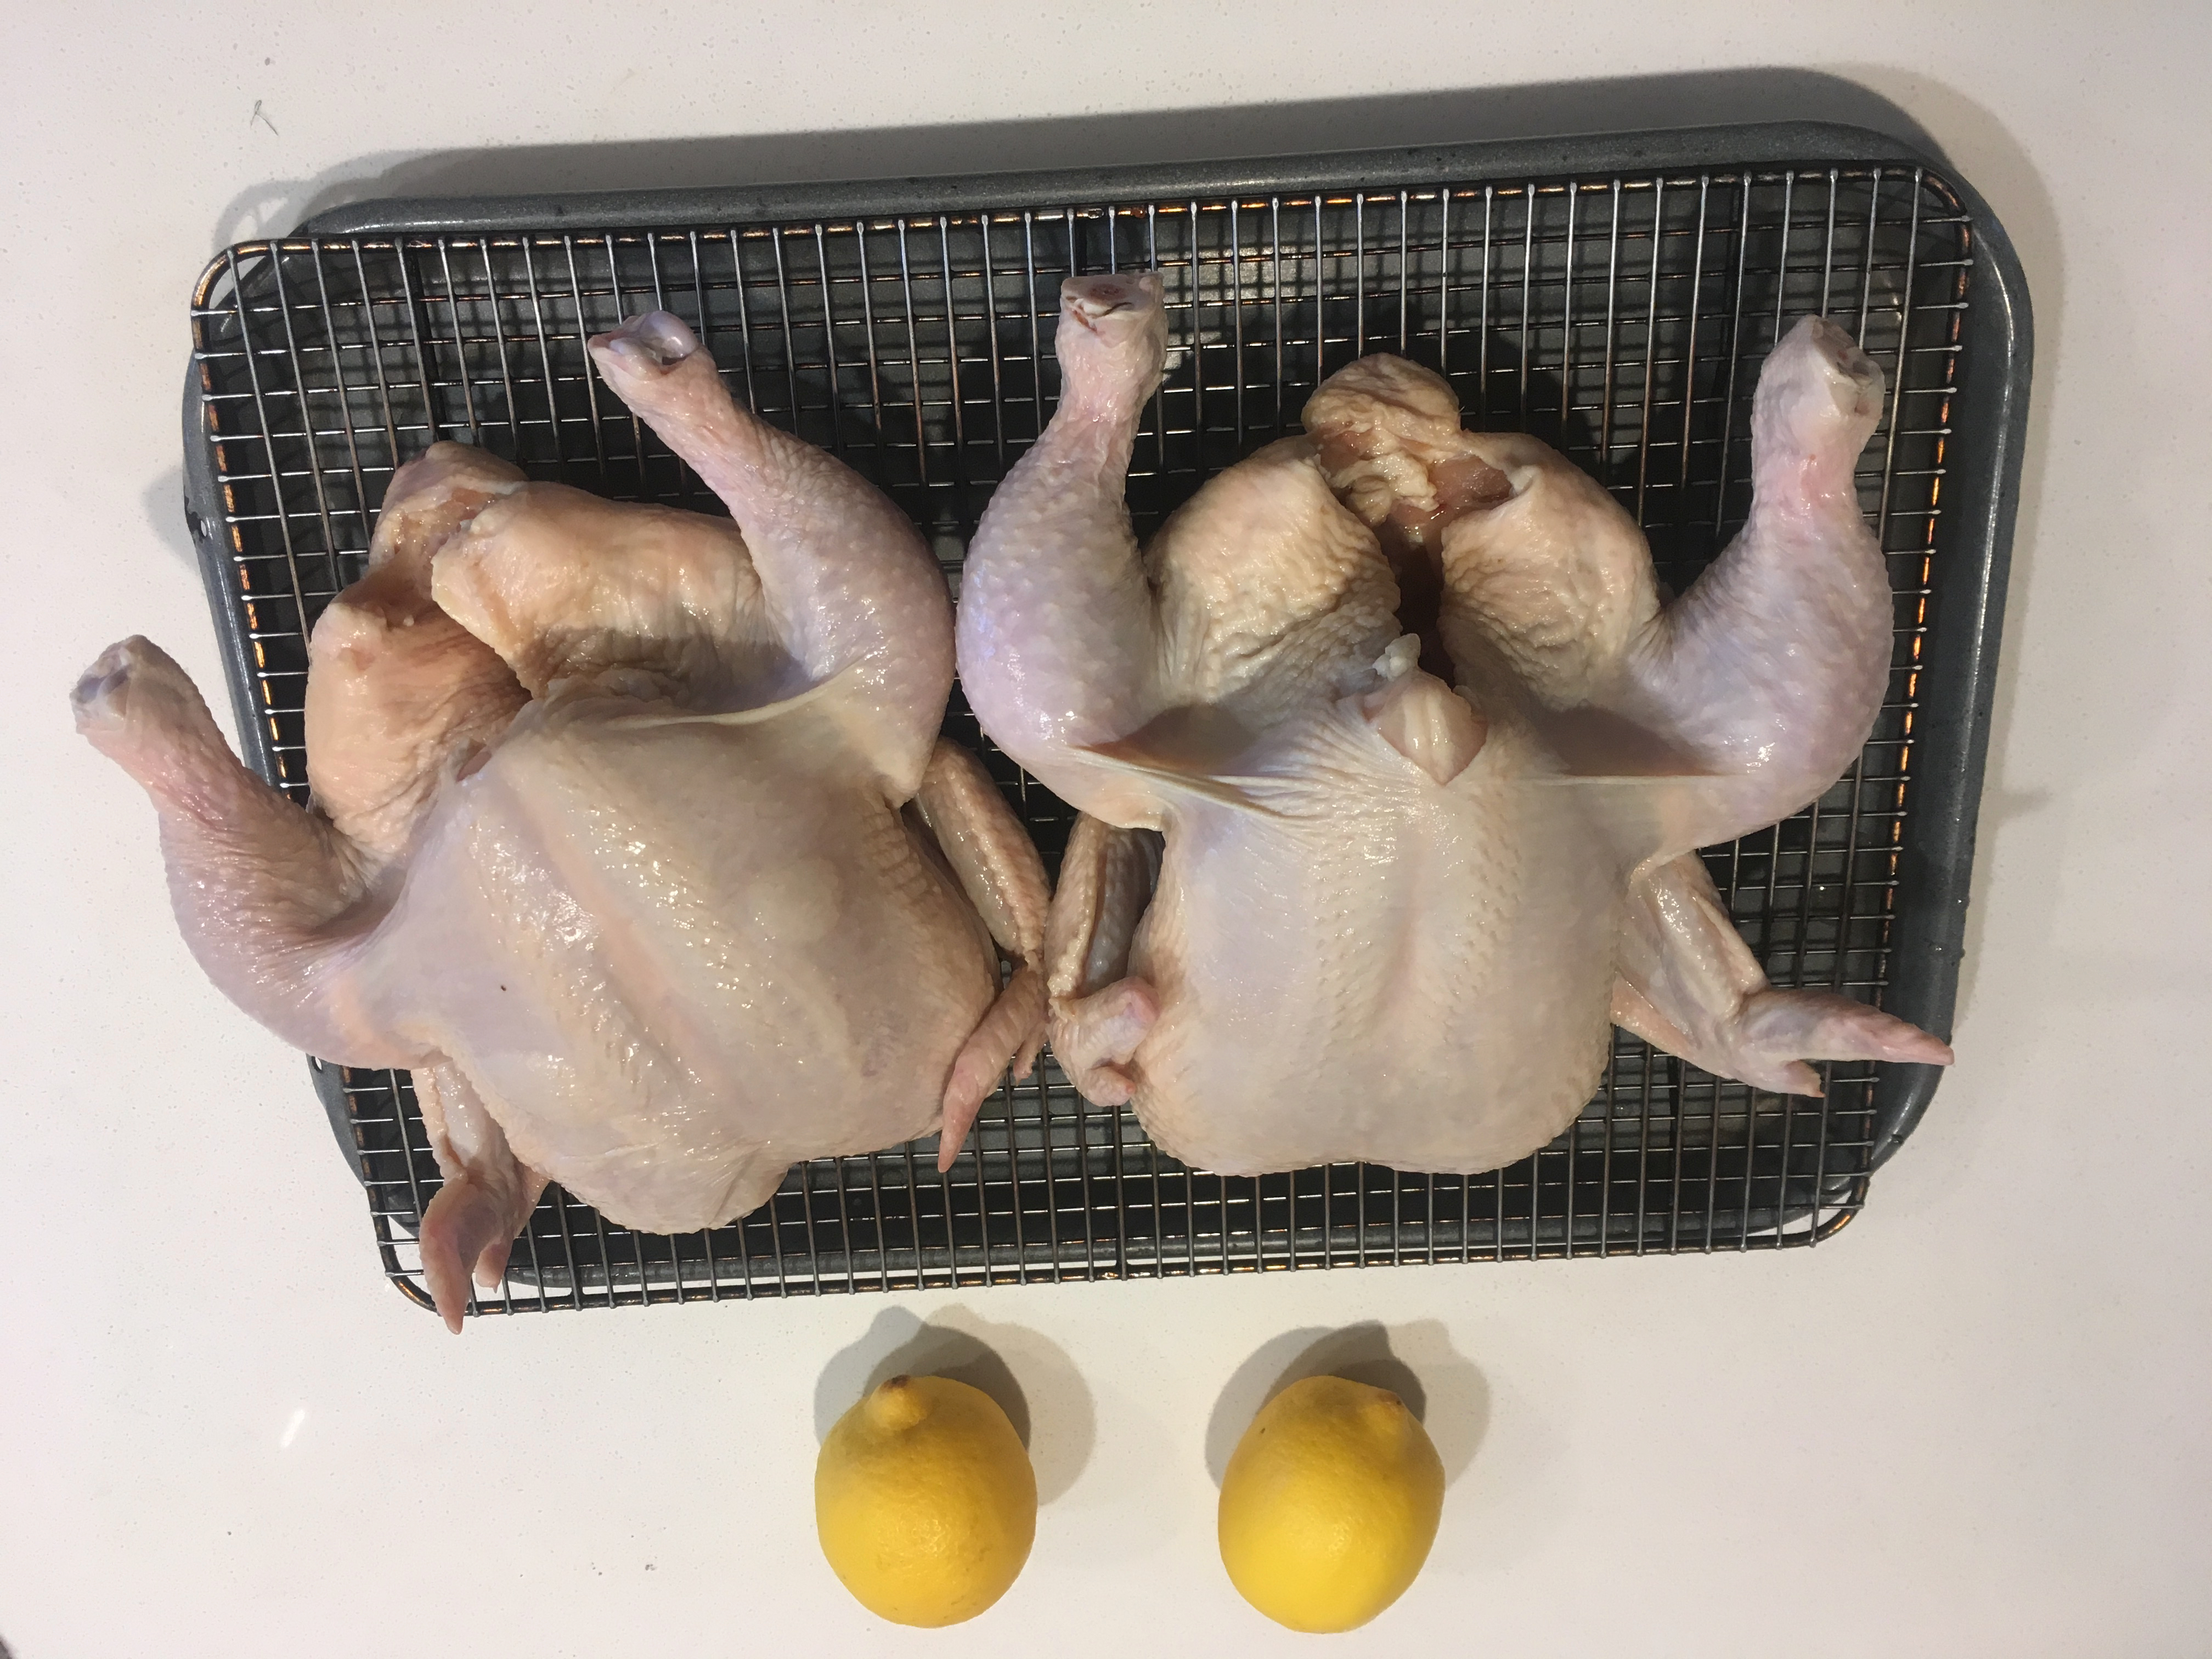
\includegraphics[width=0.25\textwidth]{\imageDir/\fileName/IMG_3197.jpg} &
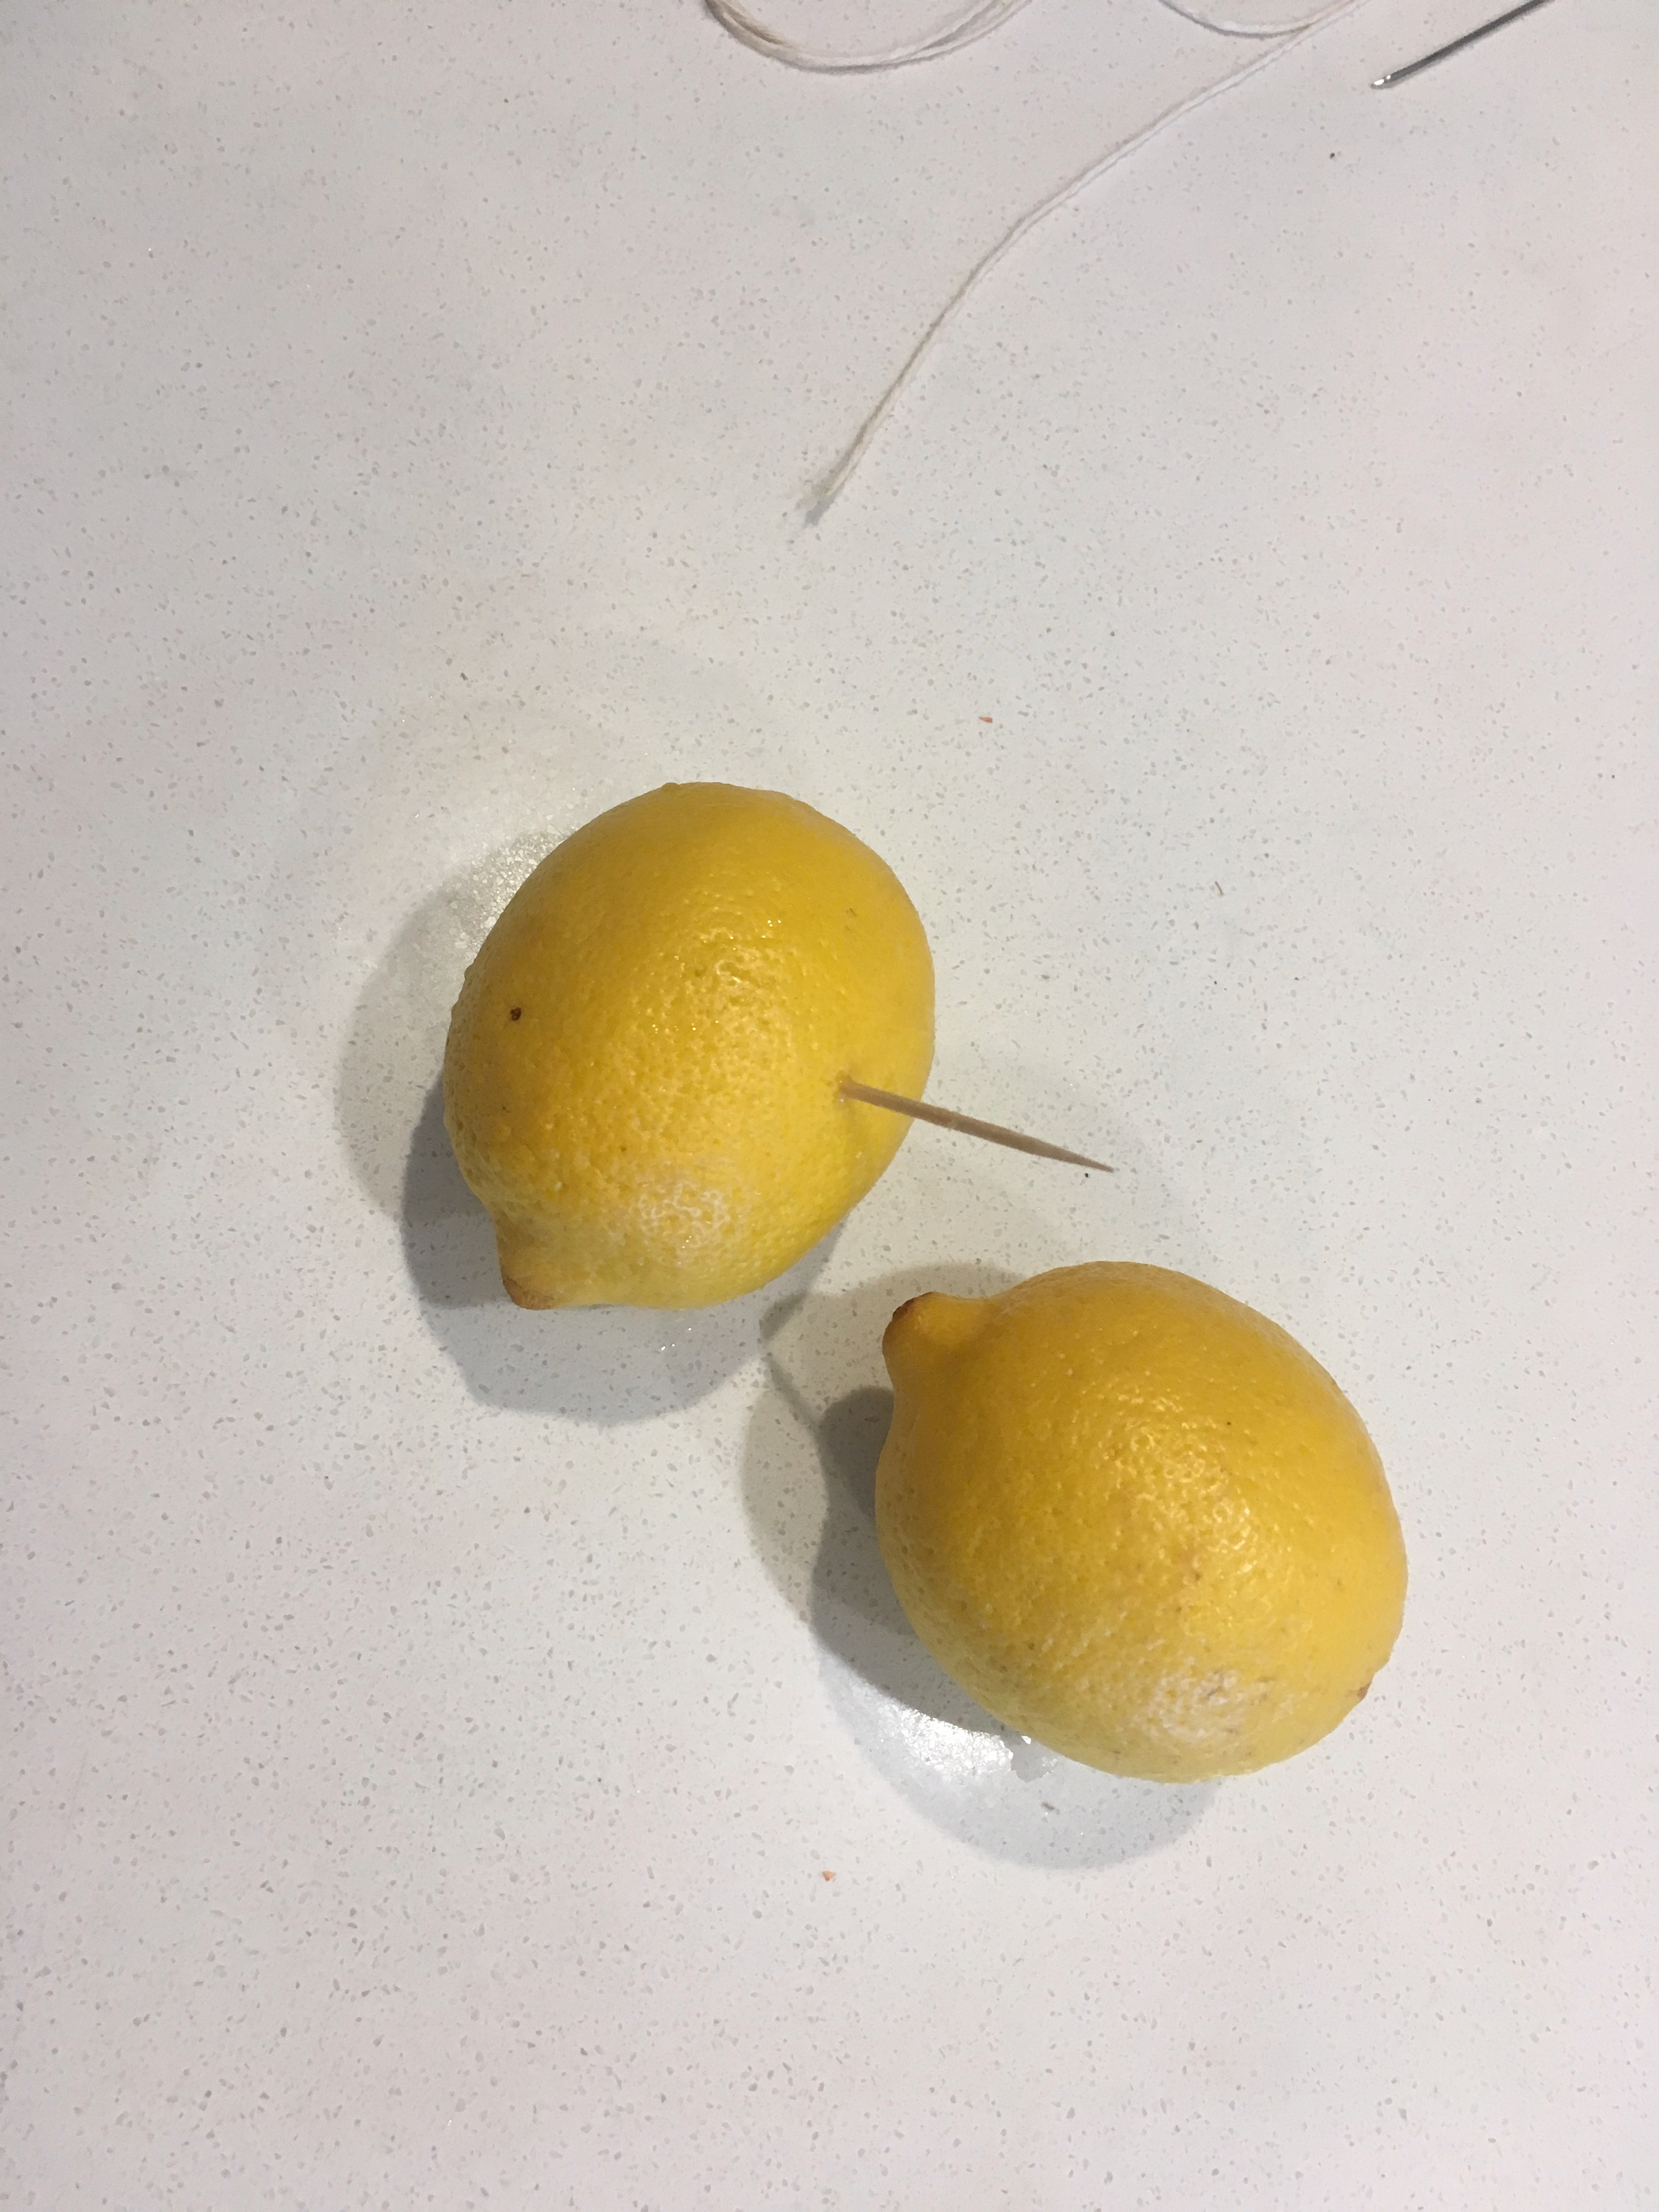
\includegraphics[width=0.25\textwidth]{\imageDir/\fileName/IMG_3212.jpg} &
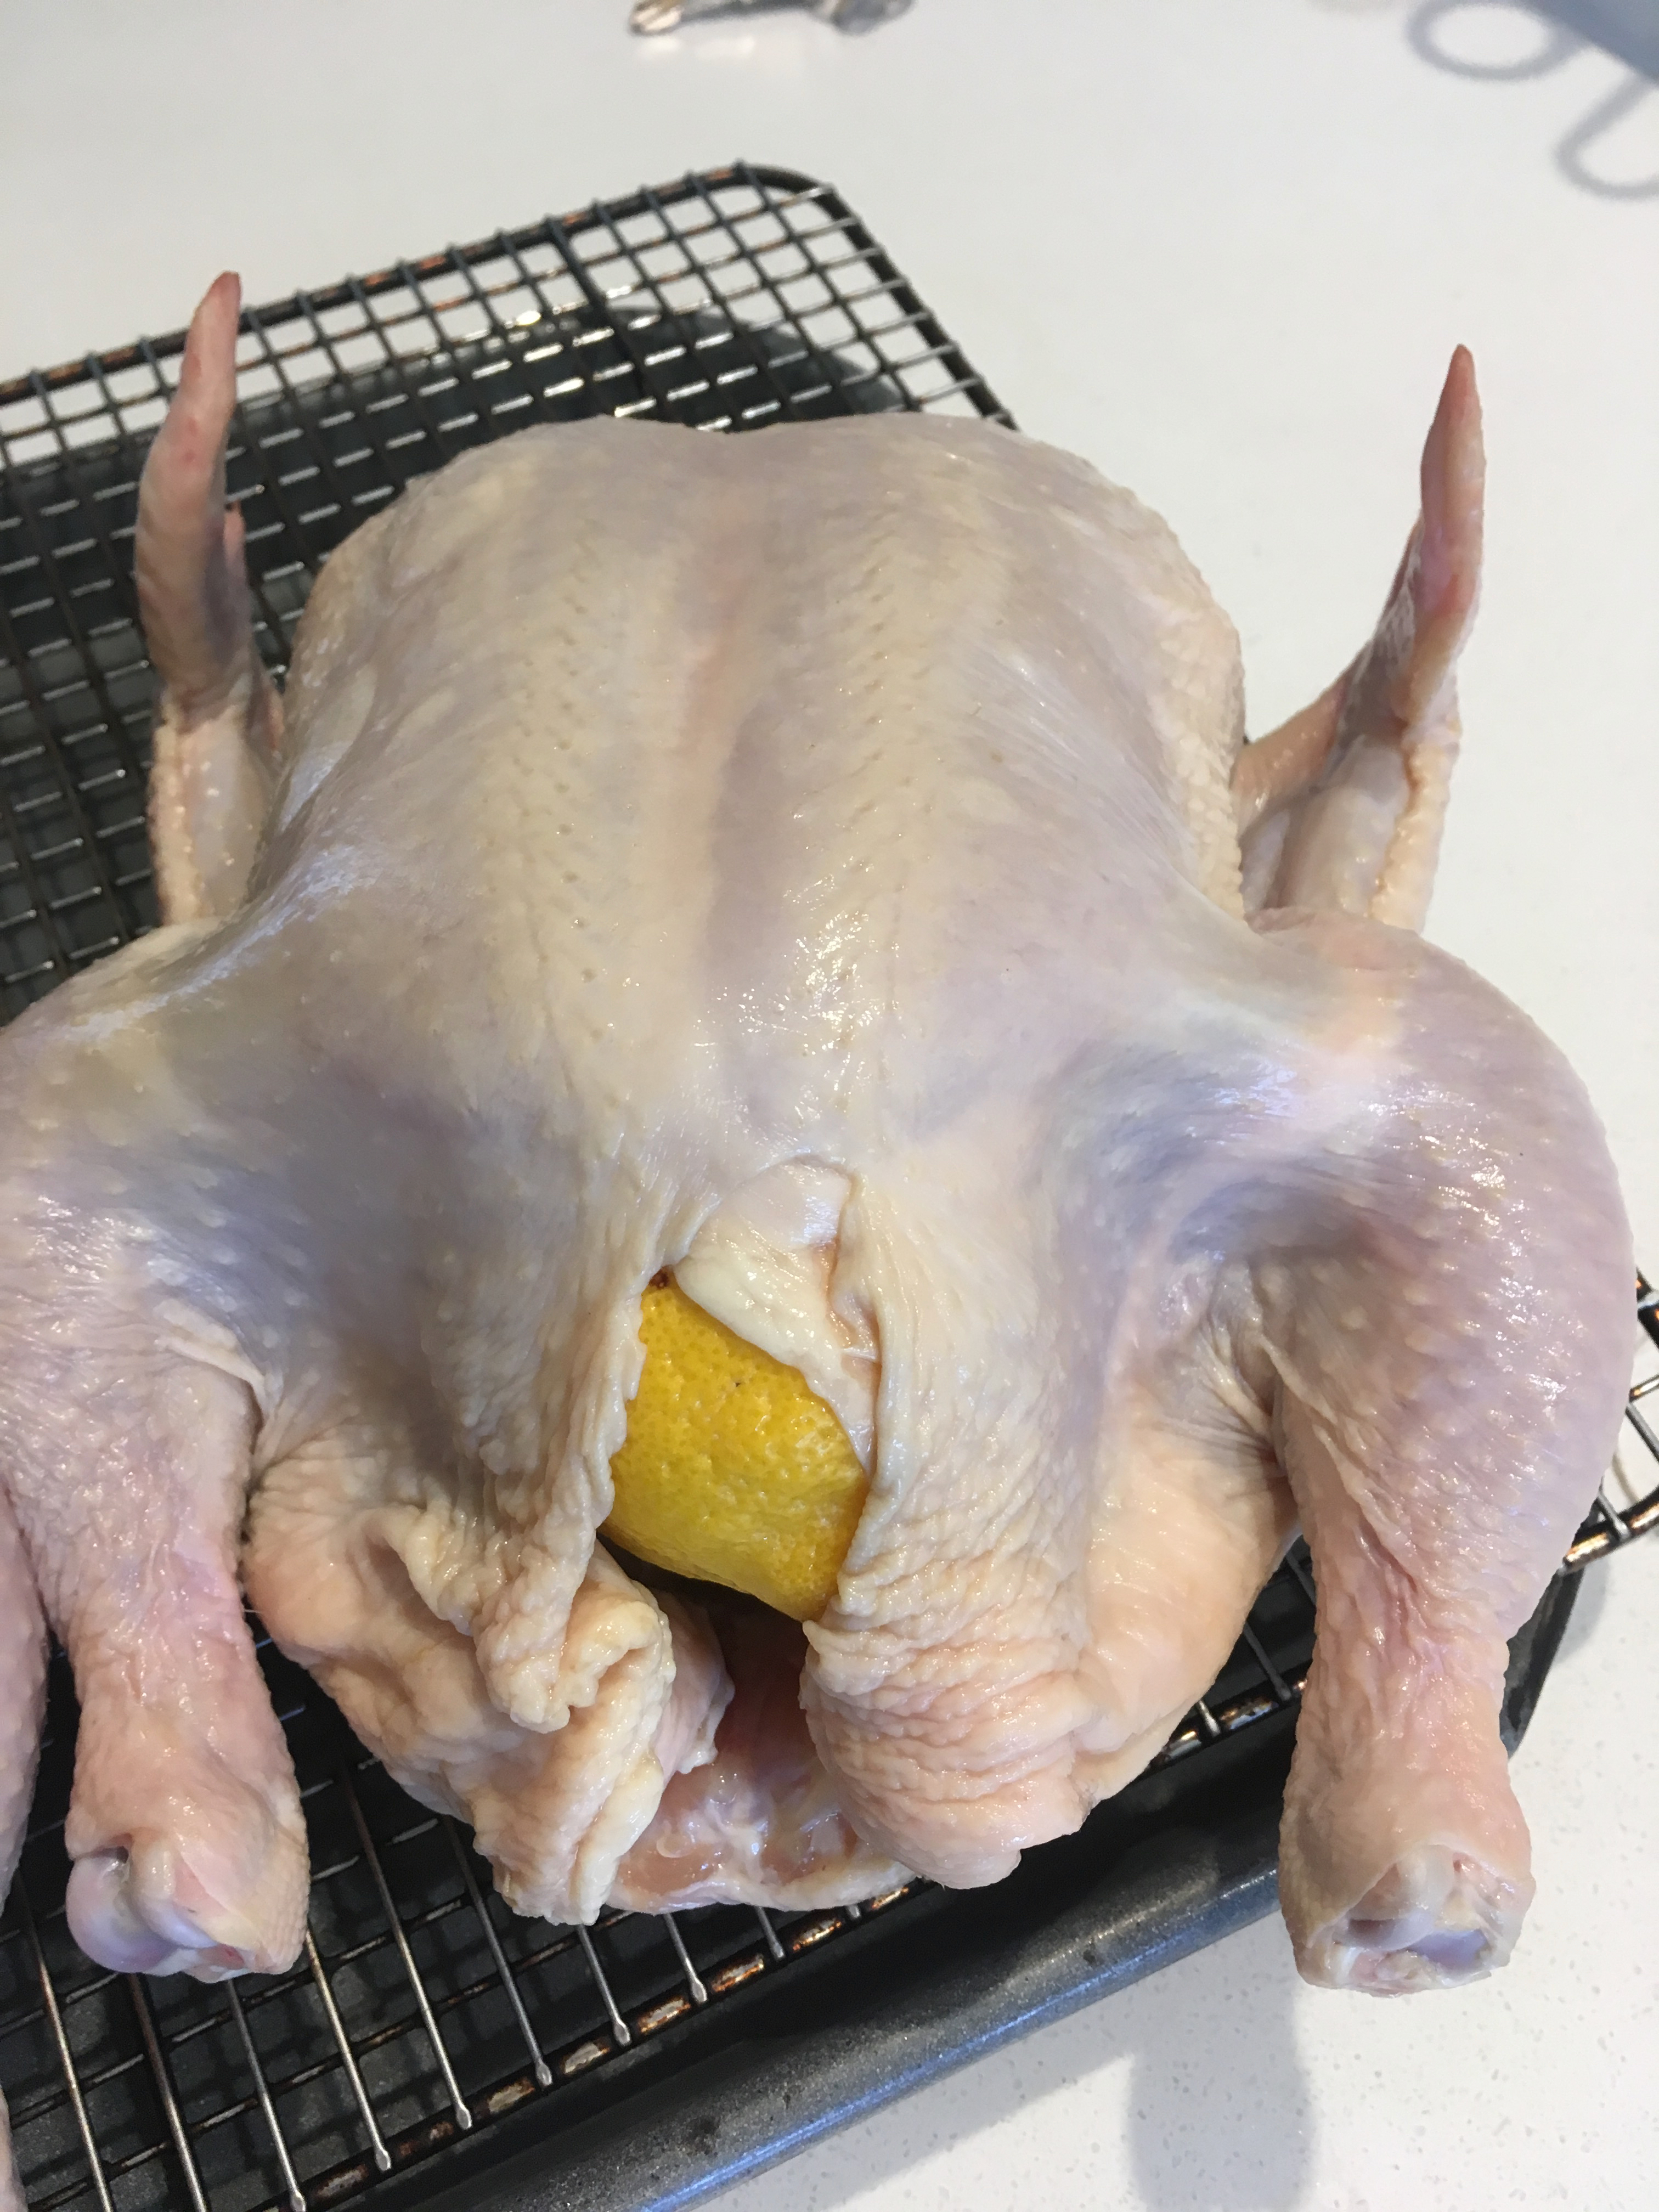
\includegraphics[width=0.25\textwidth]{\imageDir/\fileName/IMG_3213.jpg} \\
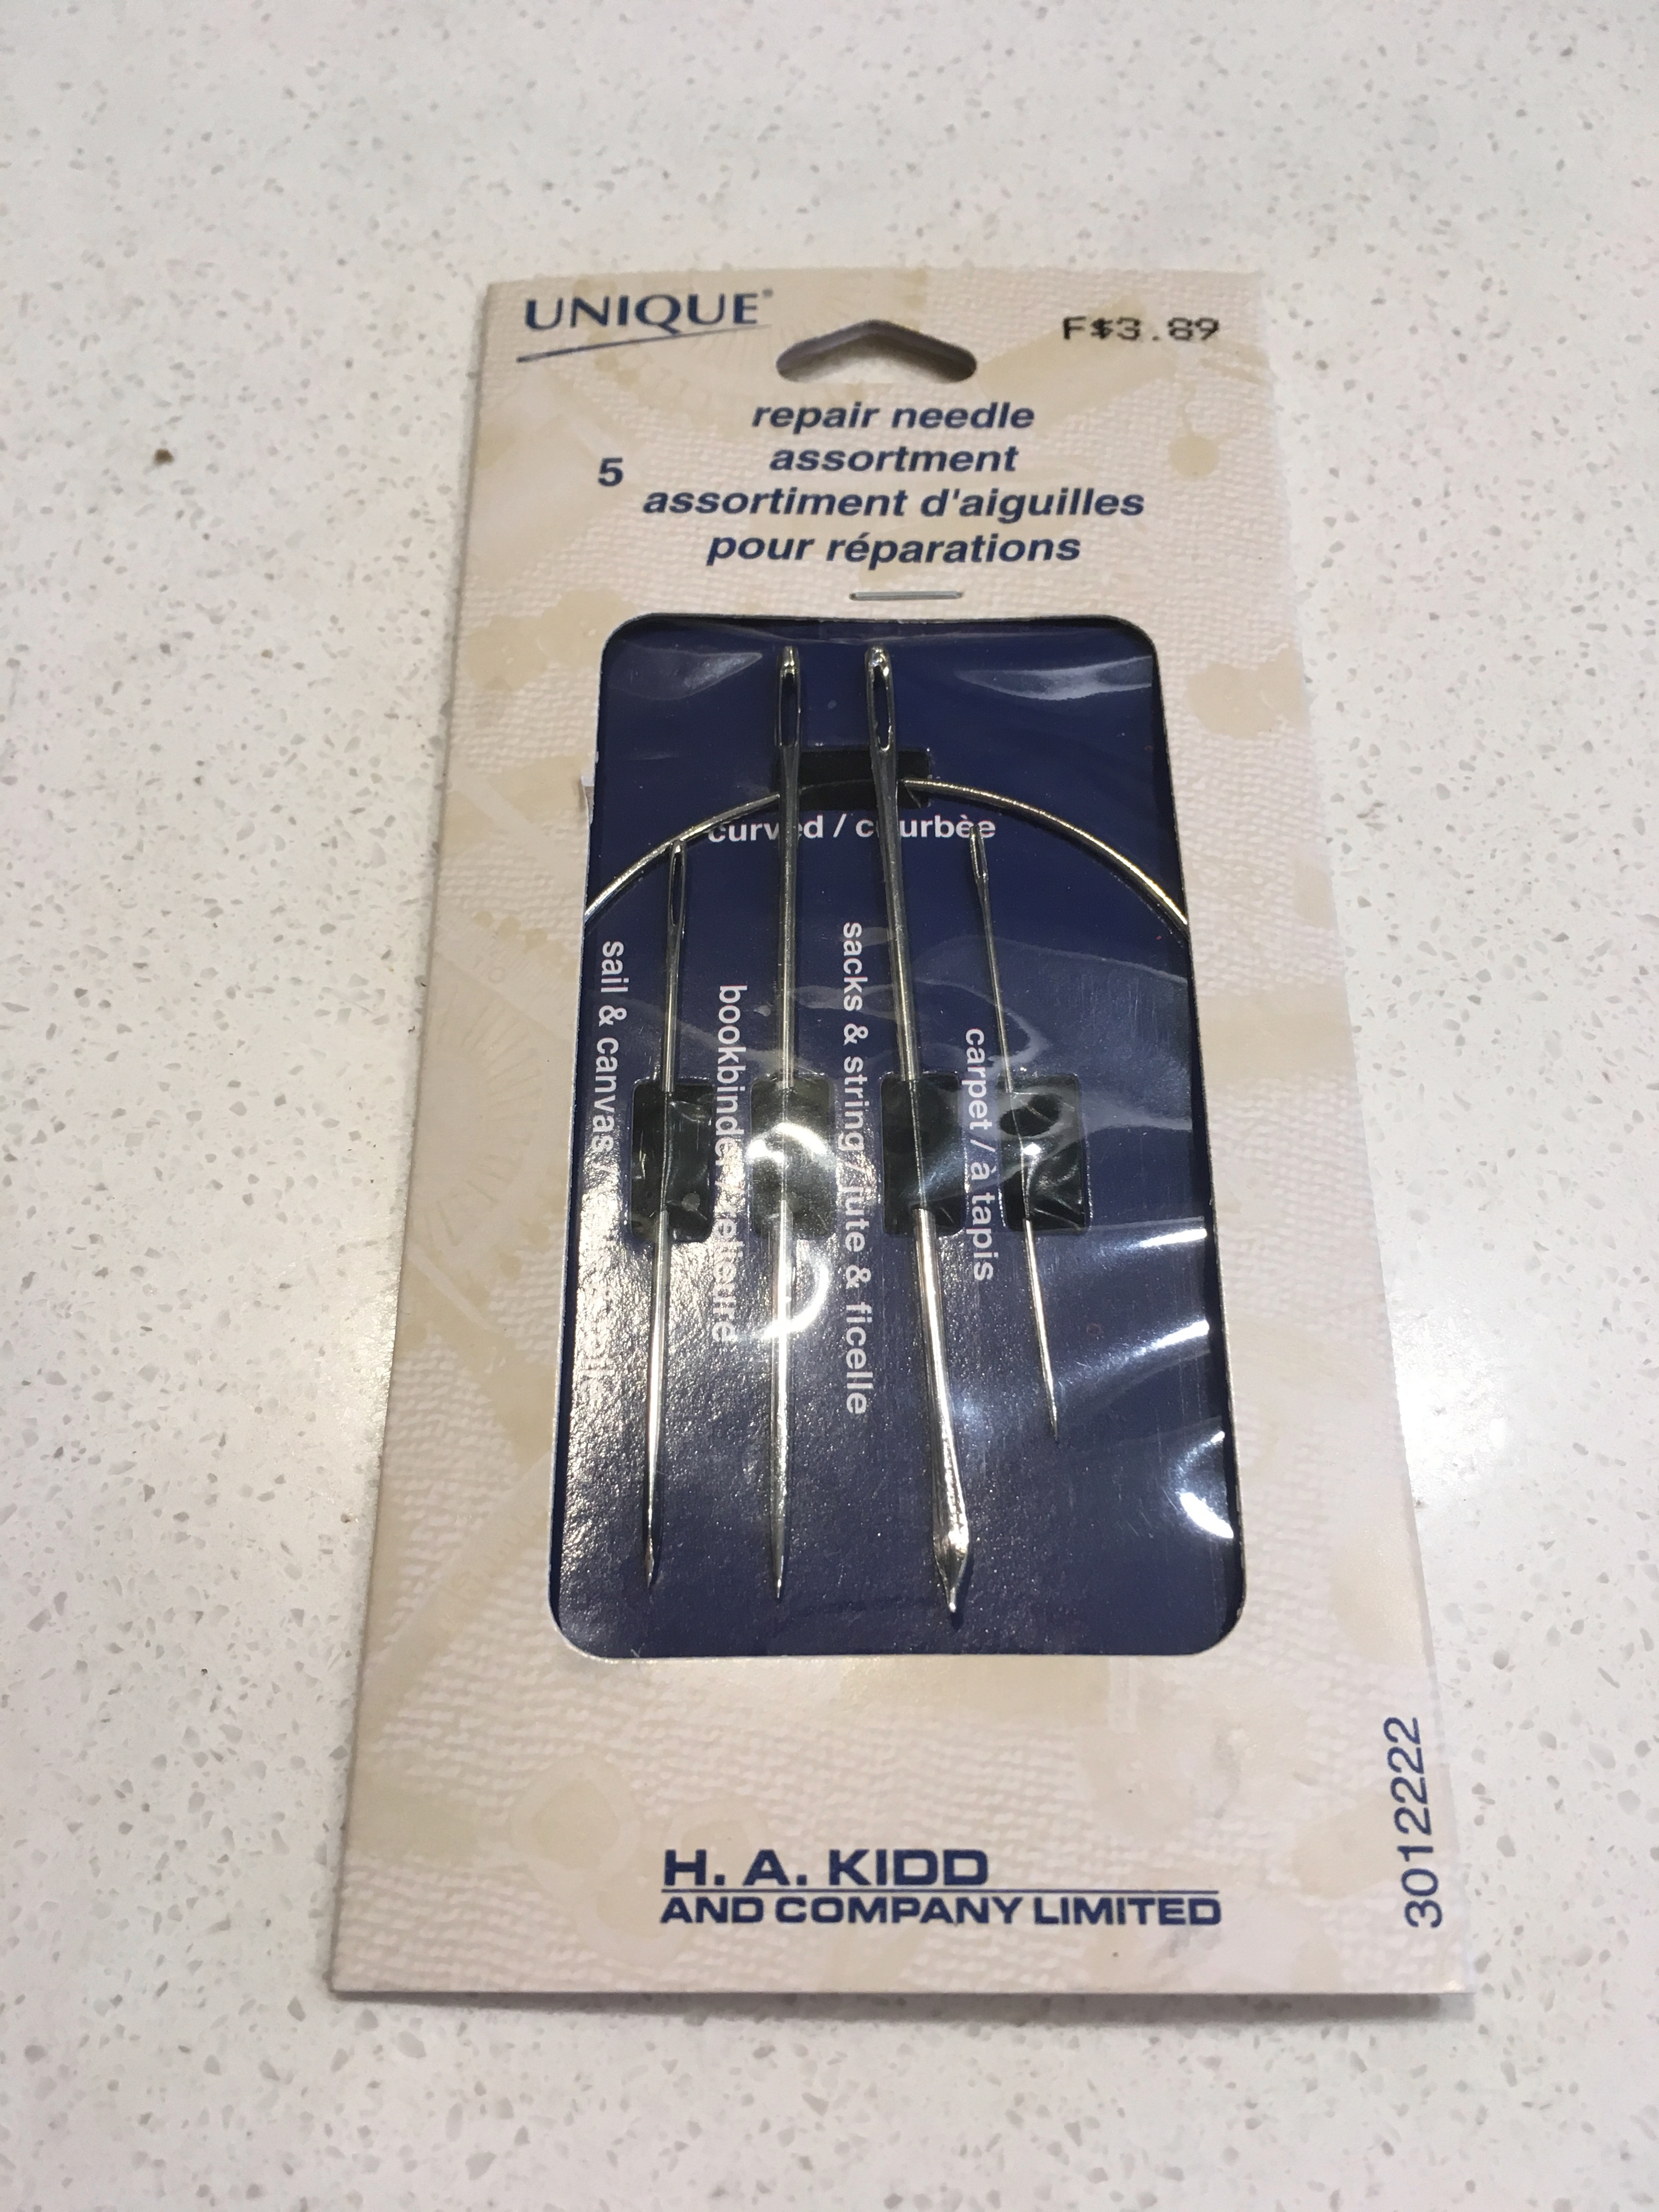
\includegraphics[width=0.25\textwidth]{\imageDir/\fileName/IMG_3206.jpg} &
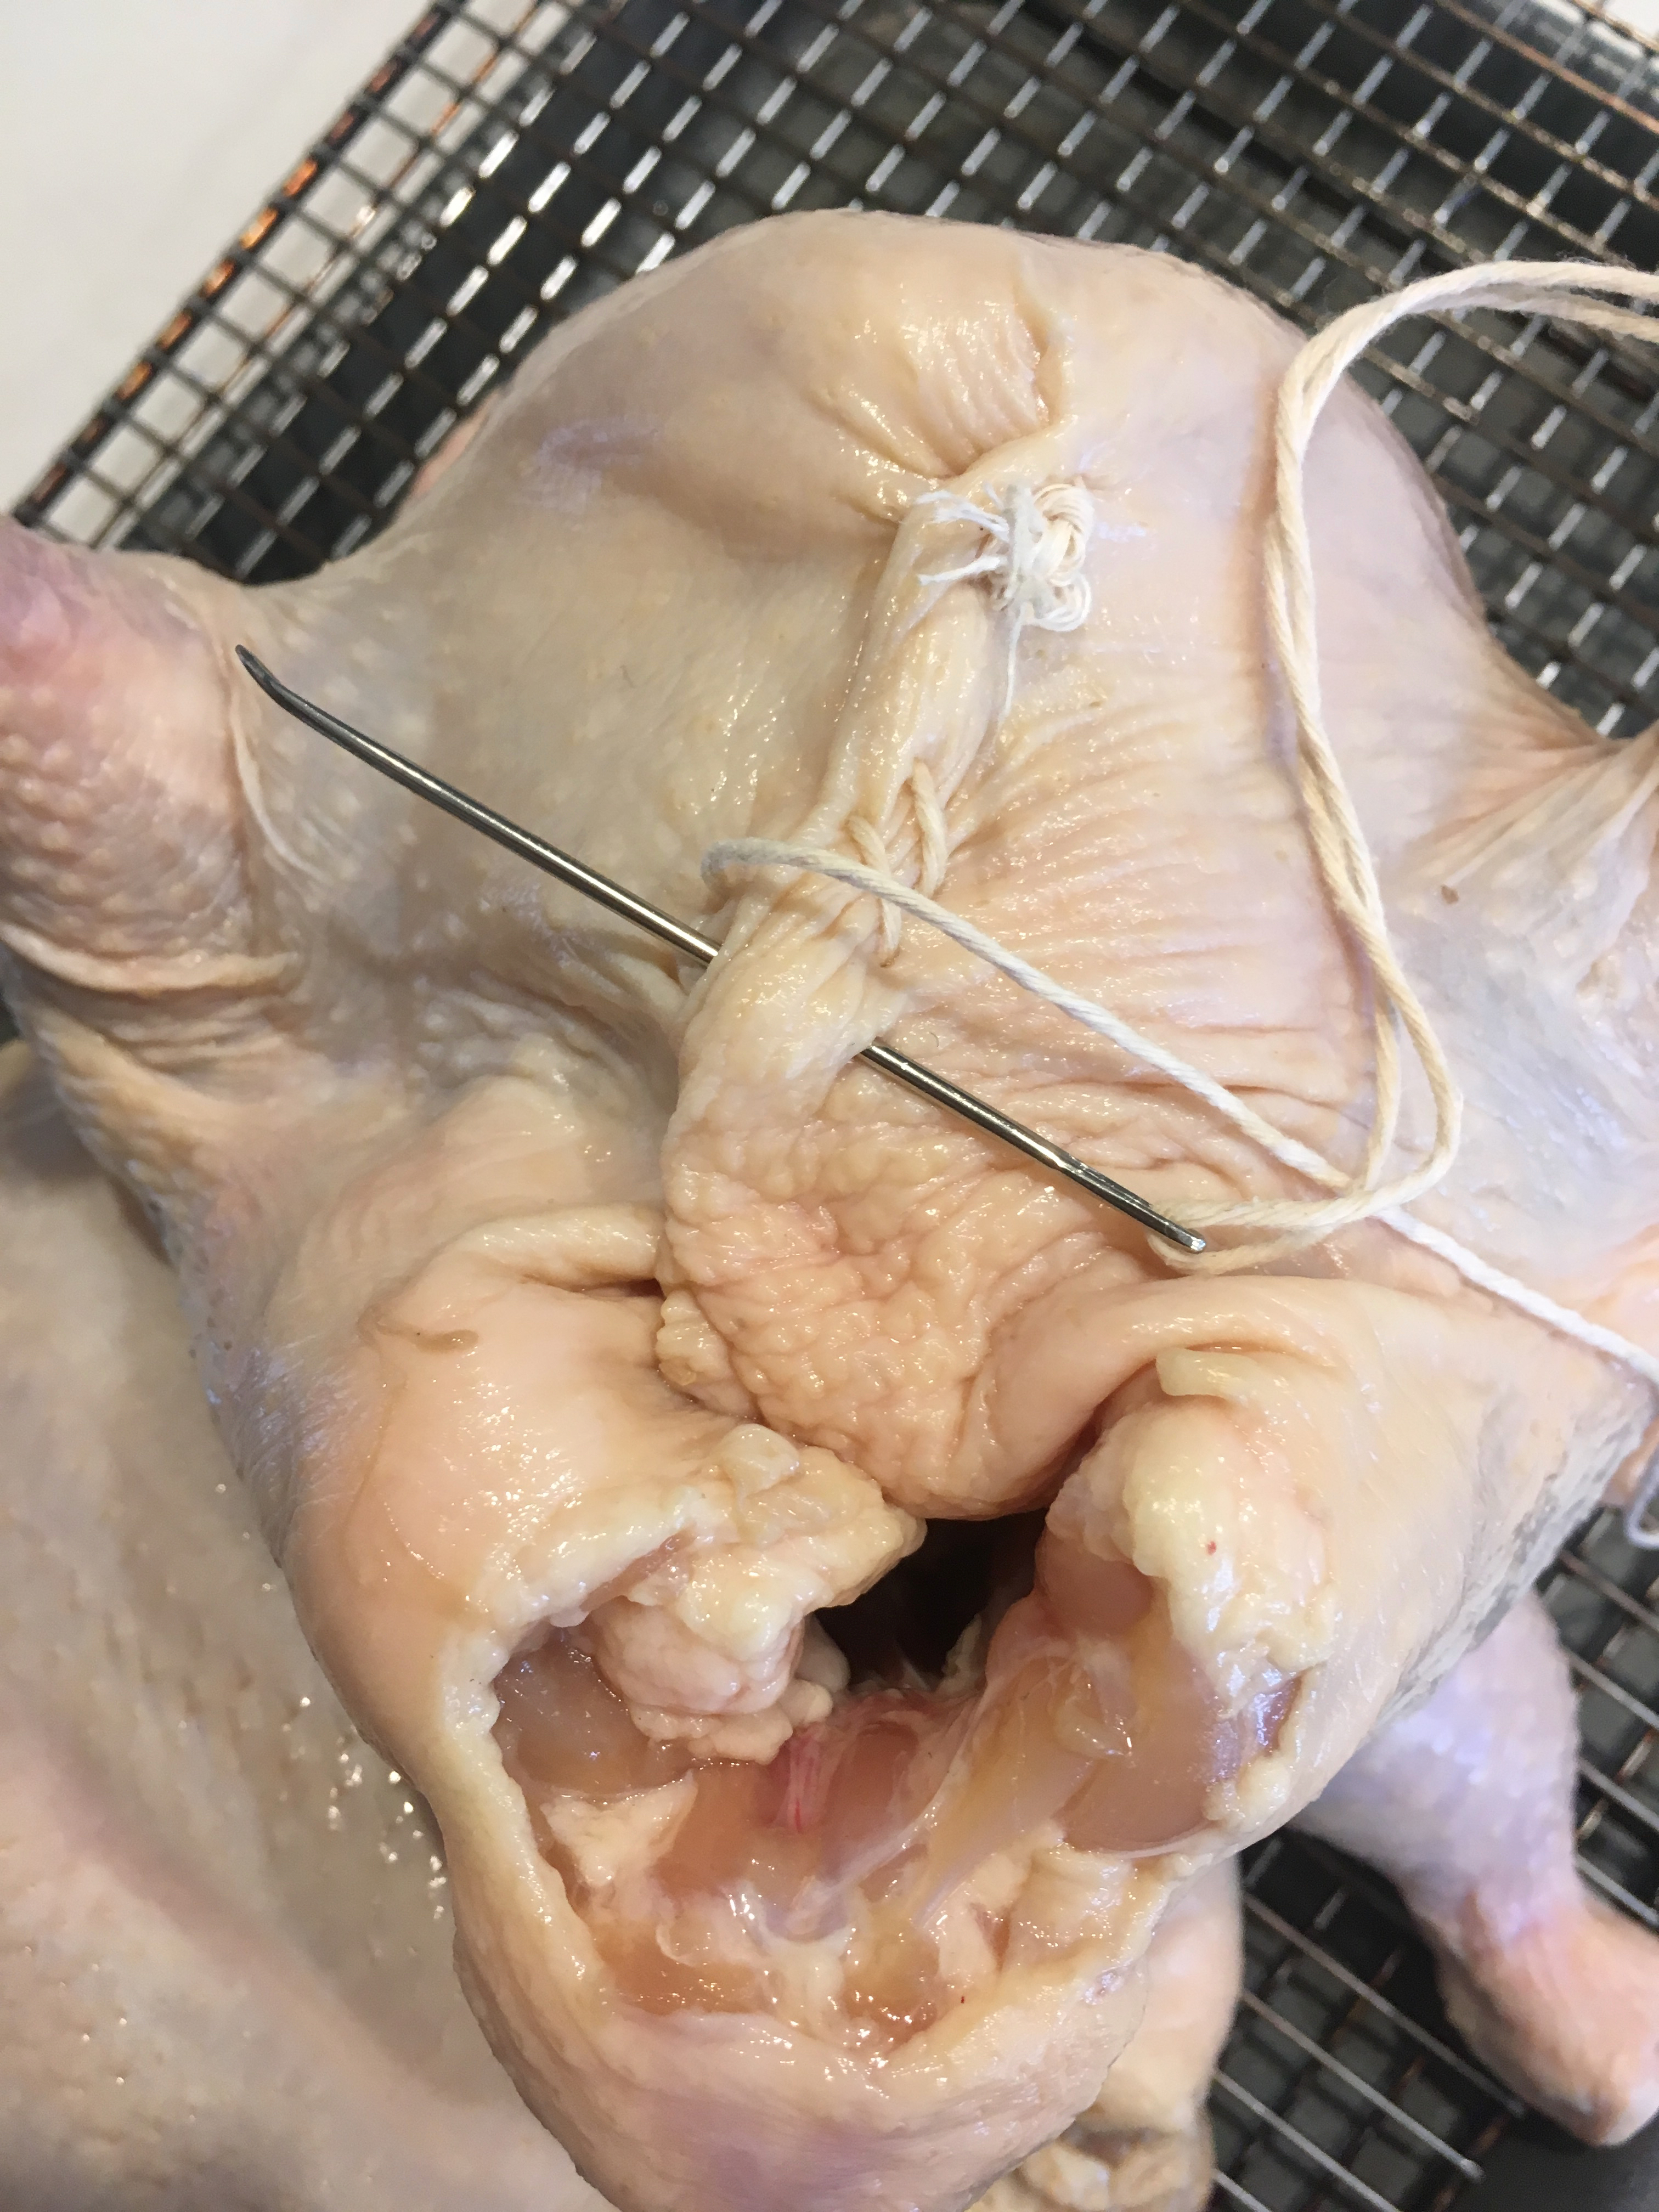
\includegraphics[width=0.25\textwidth]{\imageDir/\fileName/IMG_3214.jpg} &
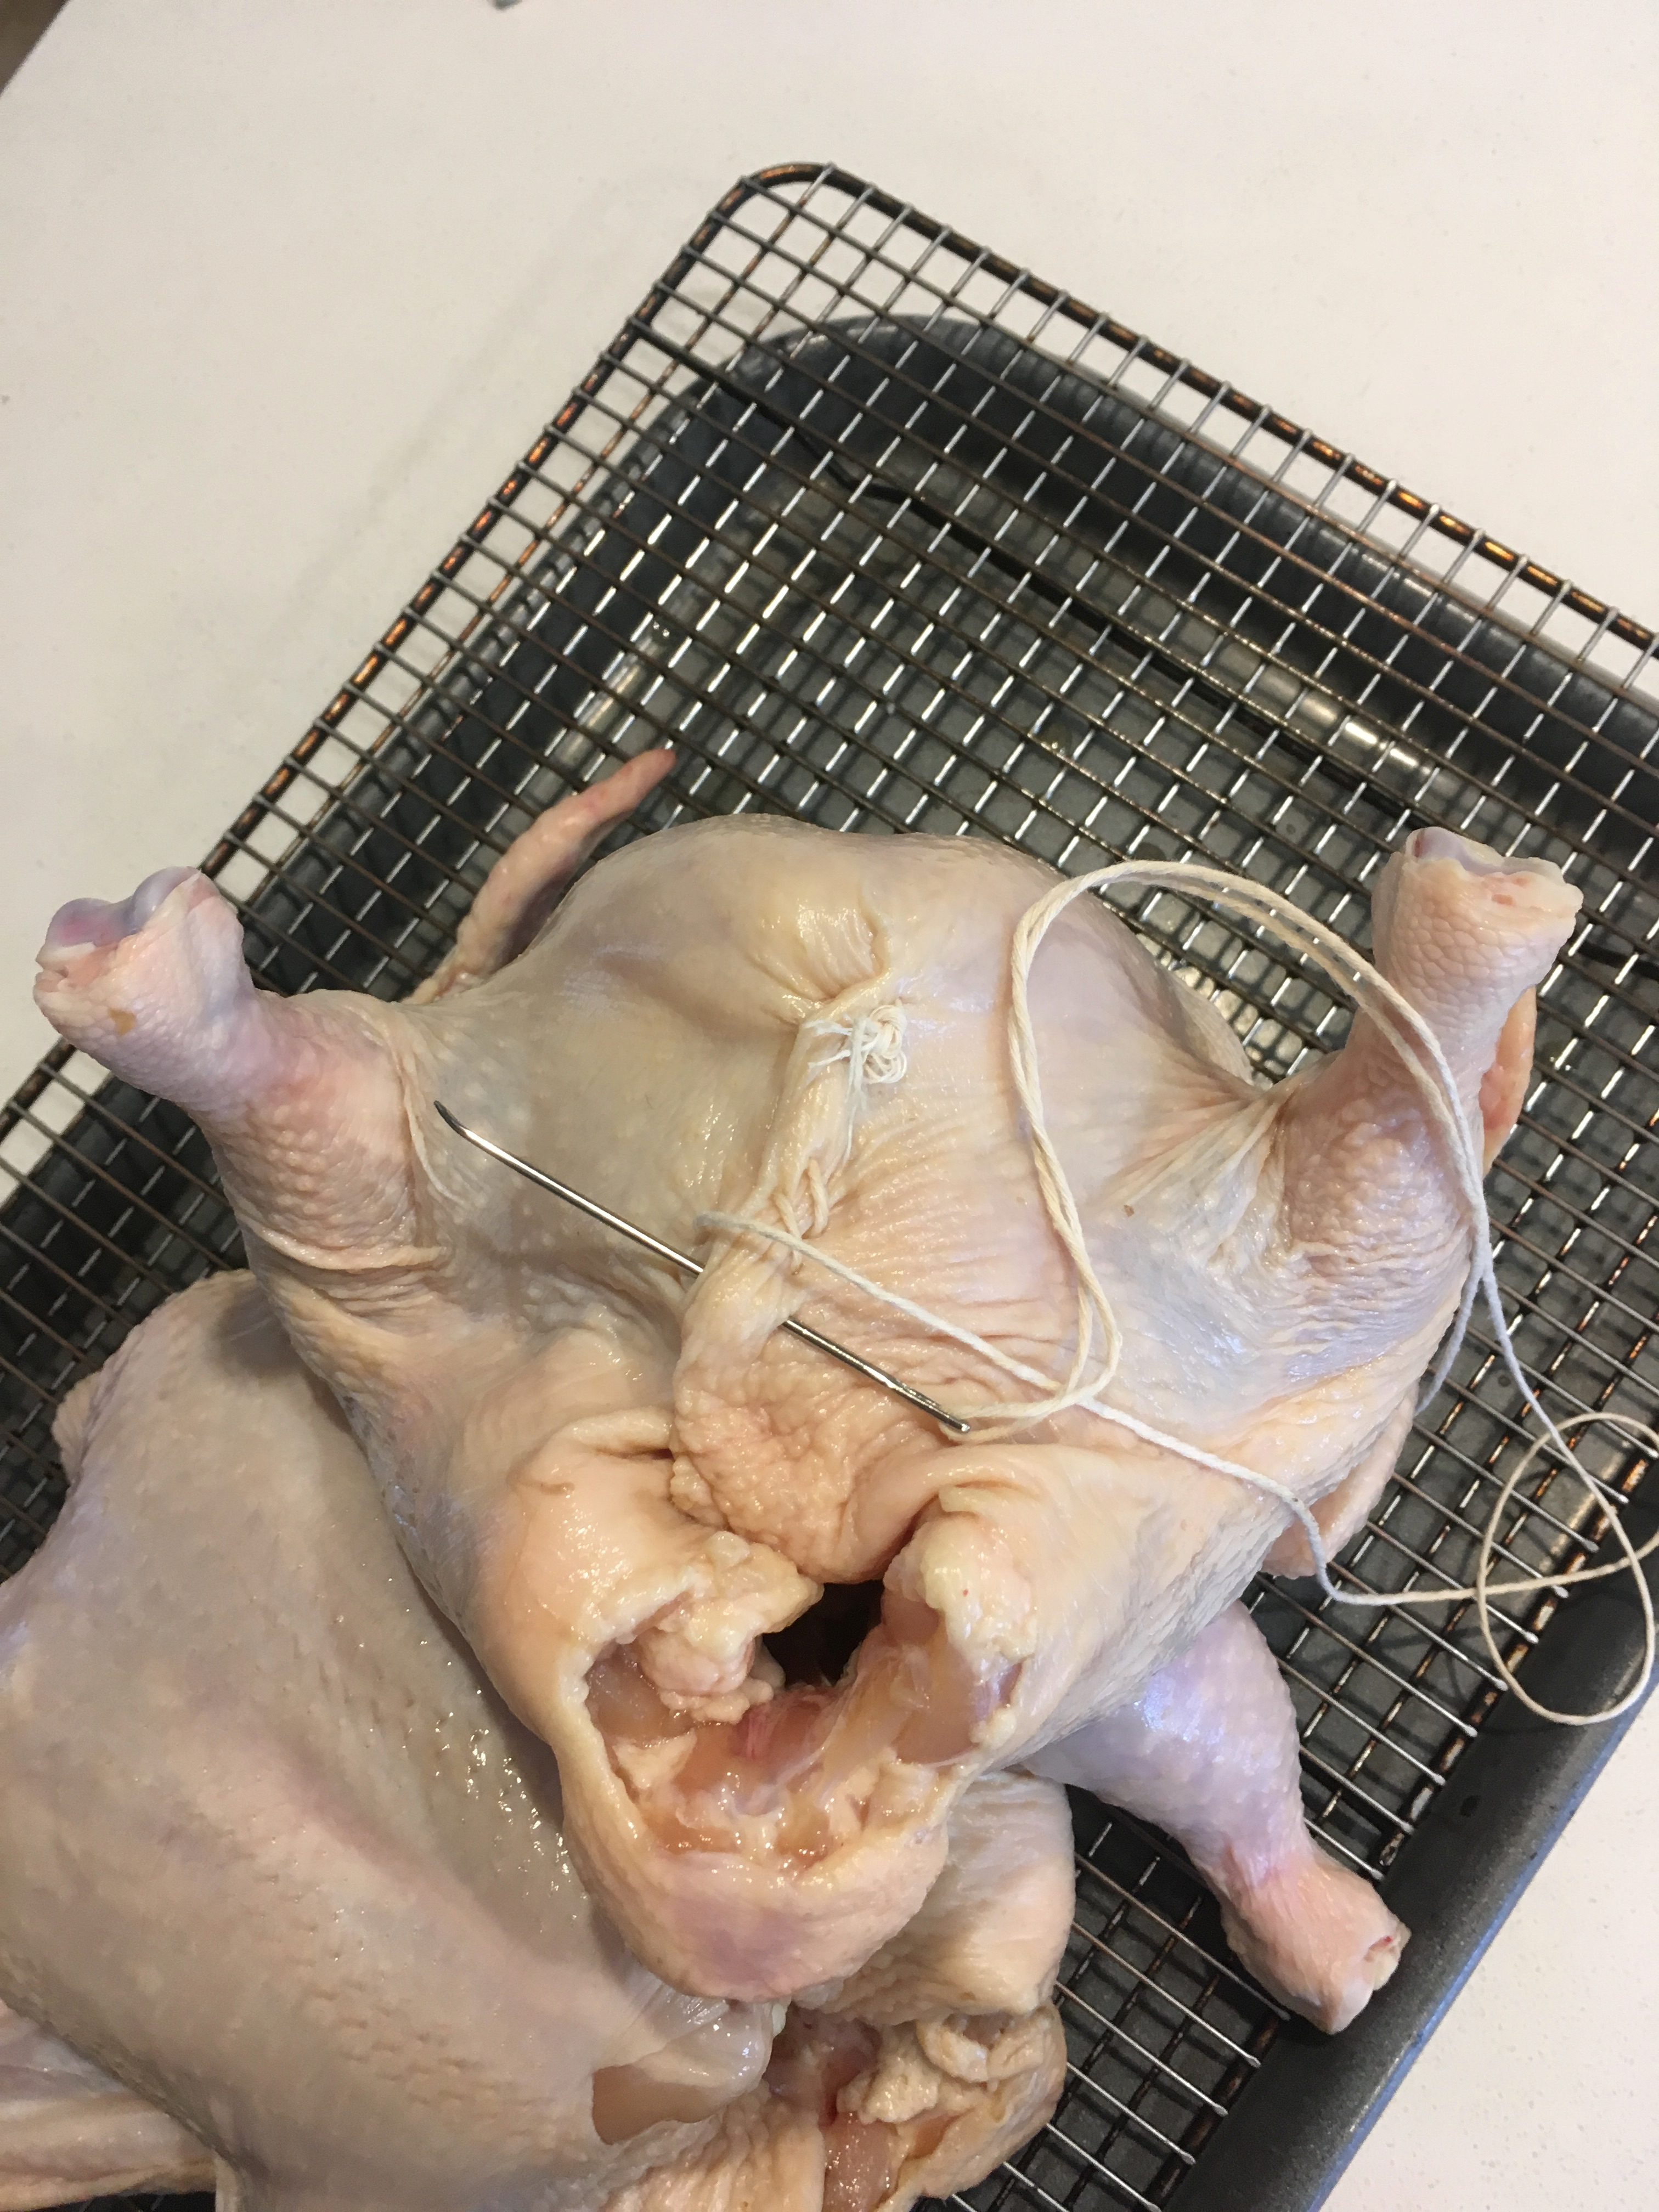
\includegraphics[width=0.25\textwidth]{\imageDir/\fileName/IMG_3216.jpg} \\
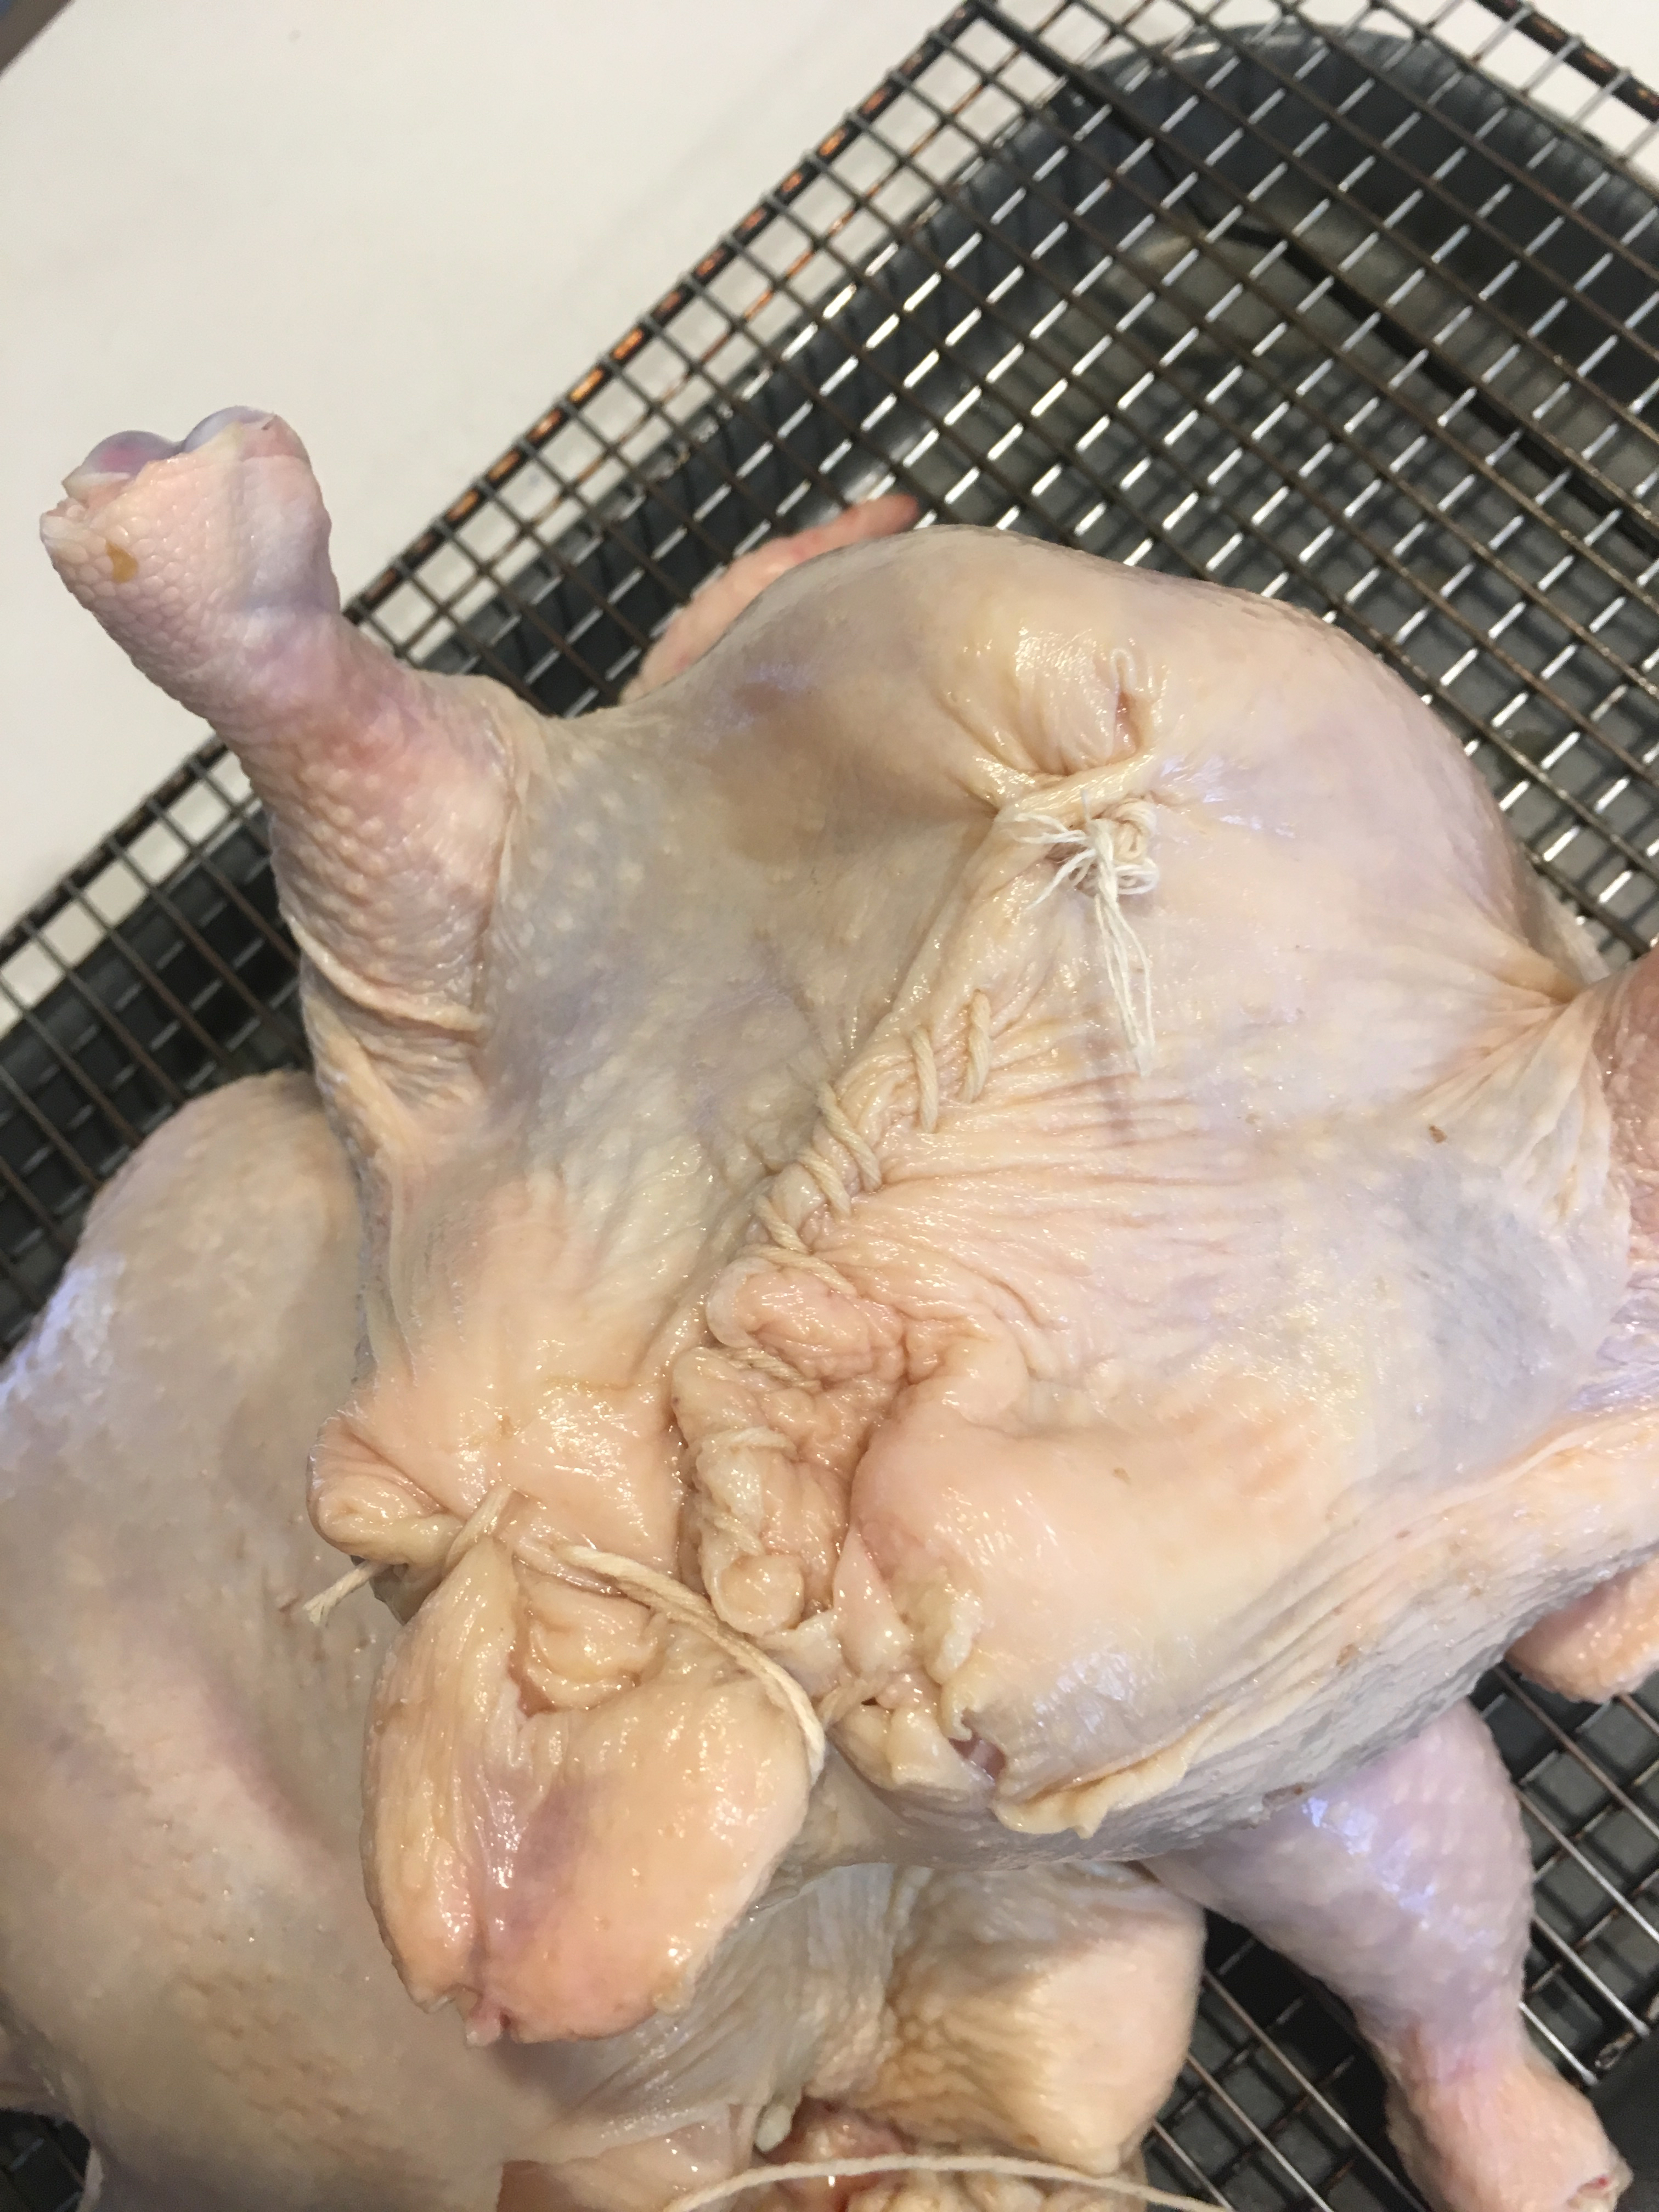
\includegraphics[width=0.25\textwidth]{\imageDir/\fileName/IMG_3217.jpg} &
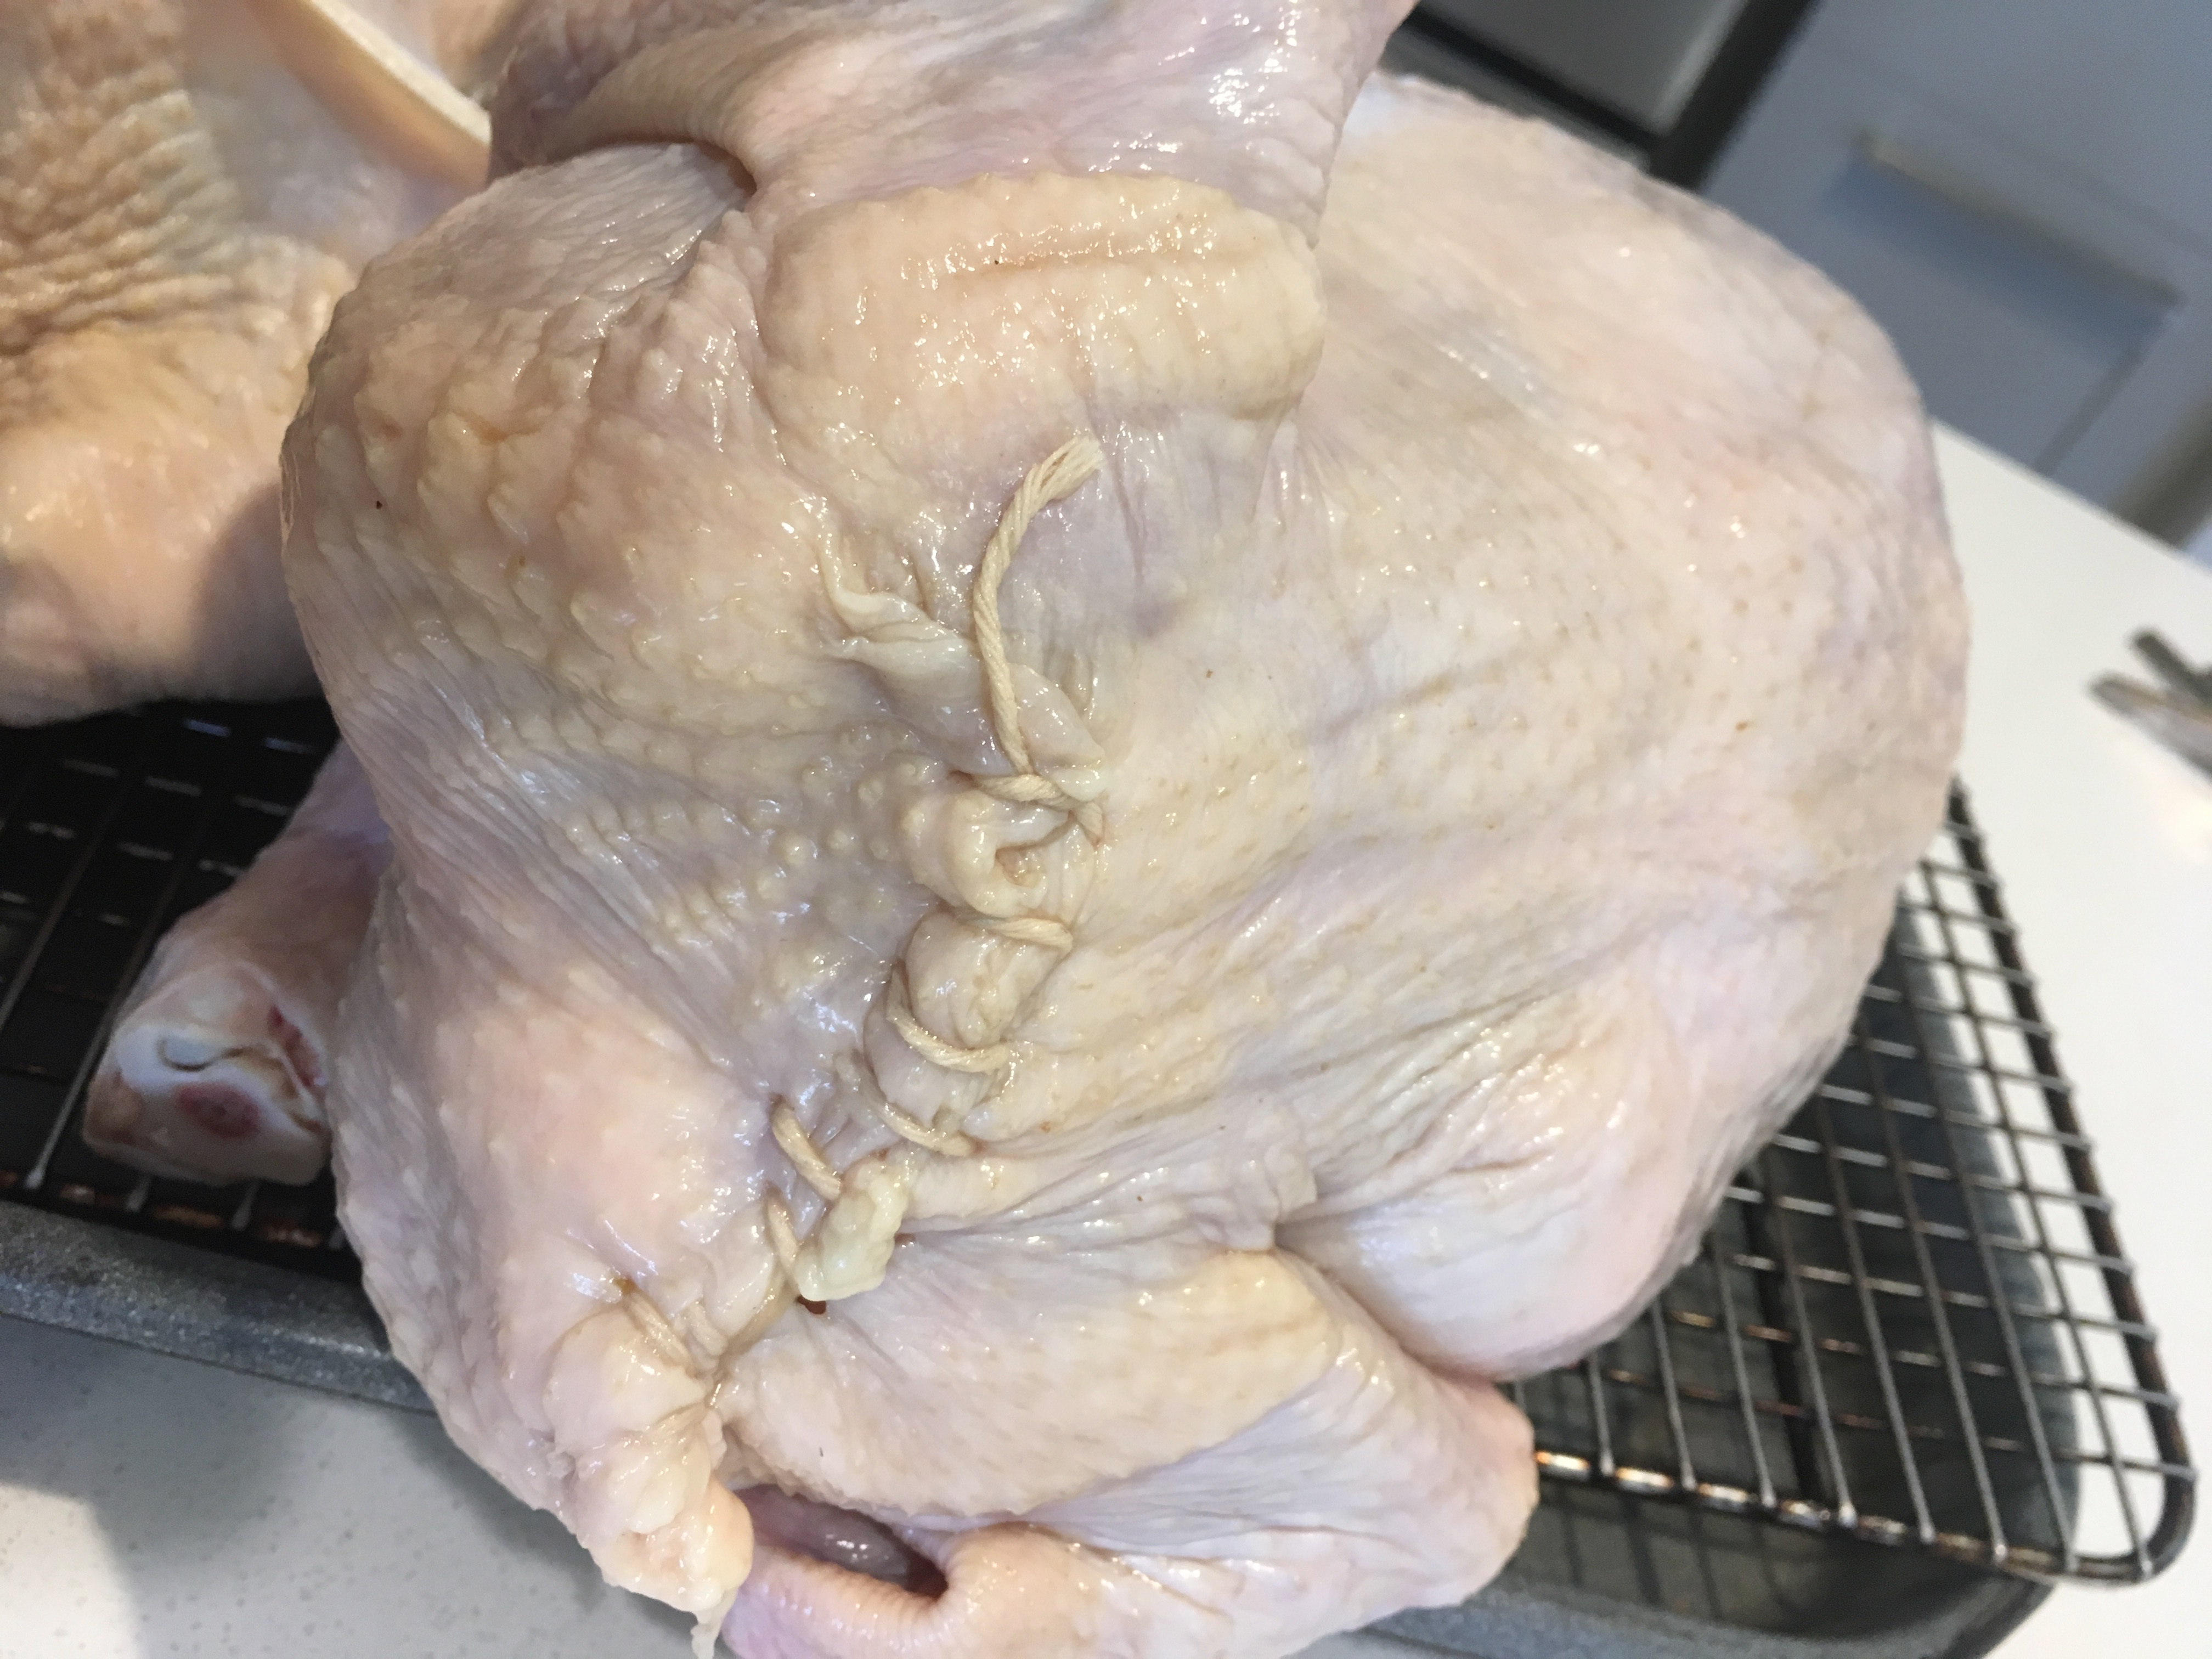
\includegraphics[width=0.25\textwidth]{\imageDir/\fileName/IMG_3218.jpg} &
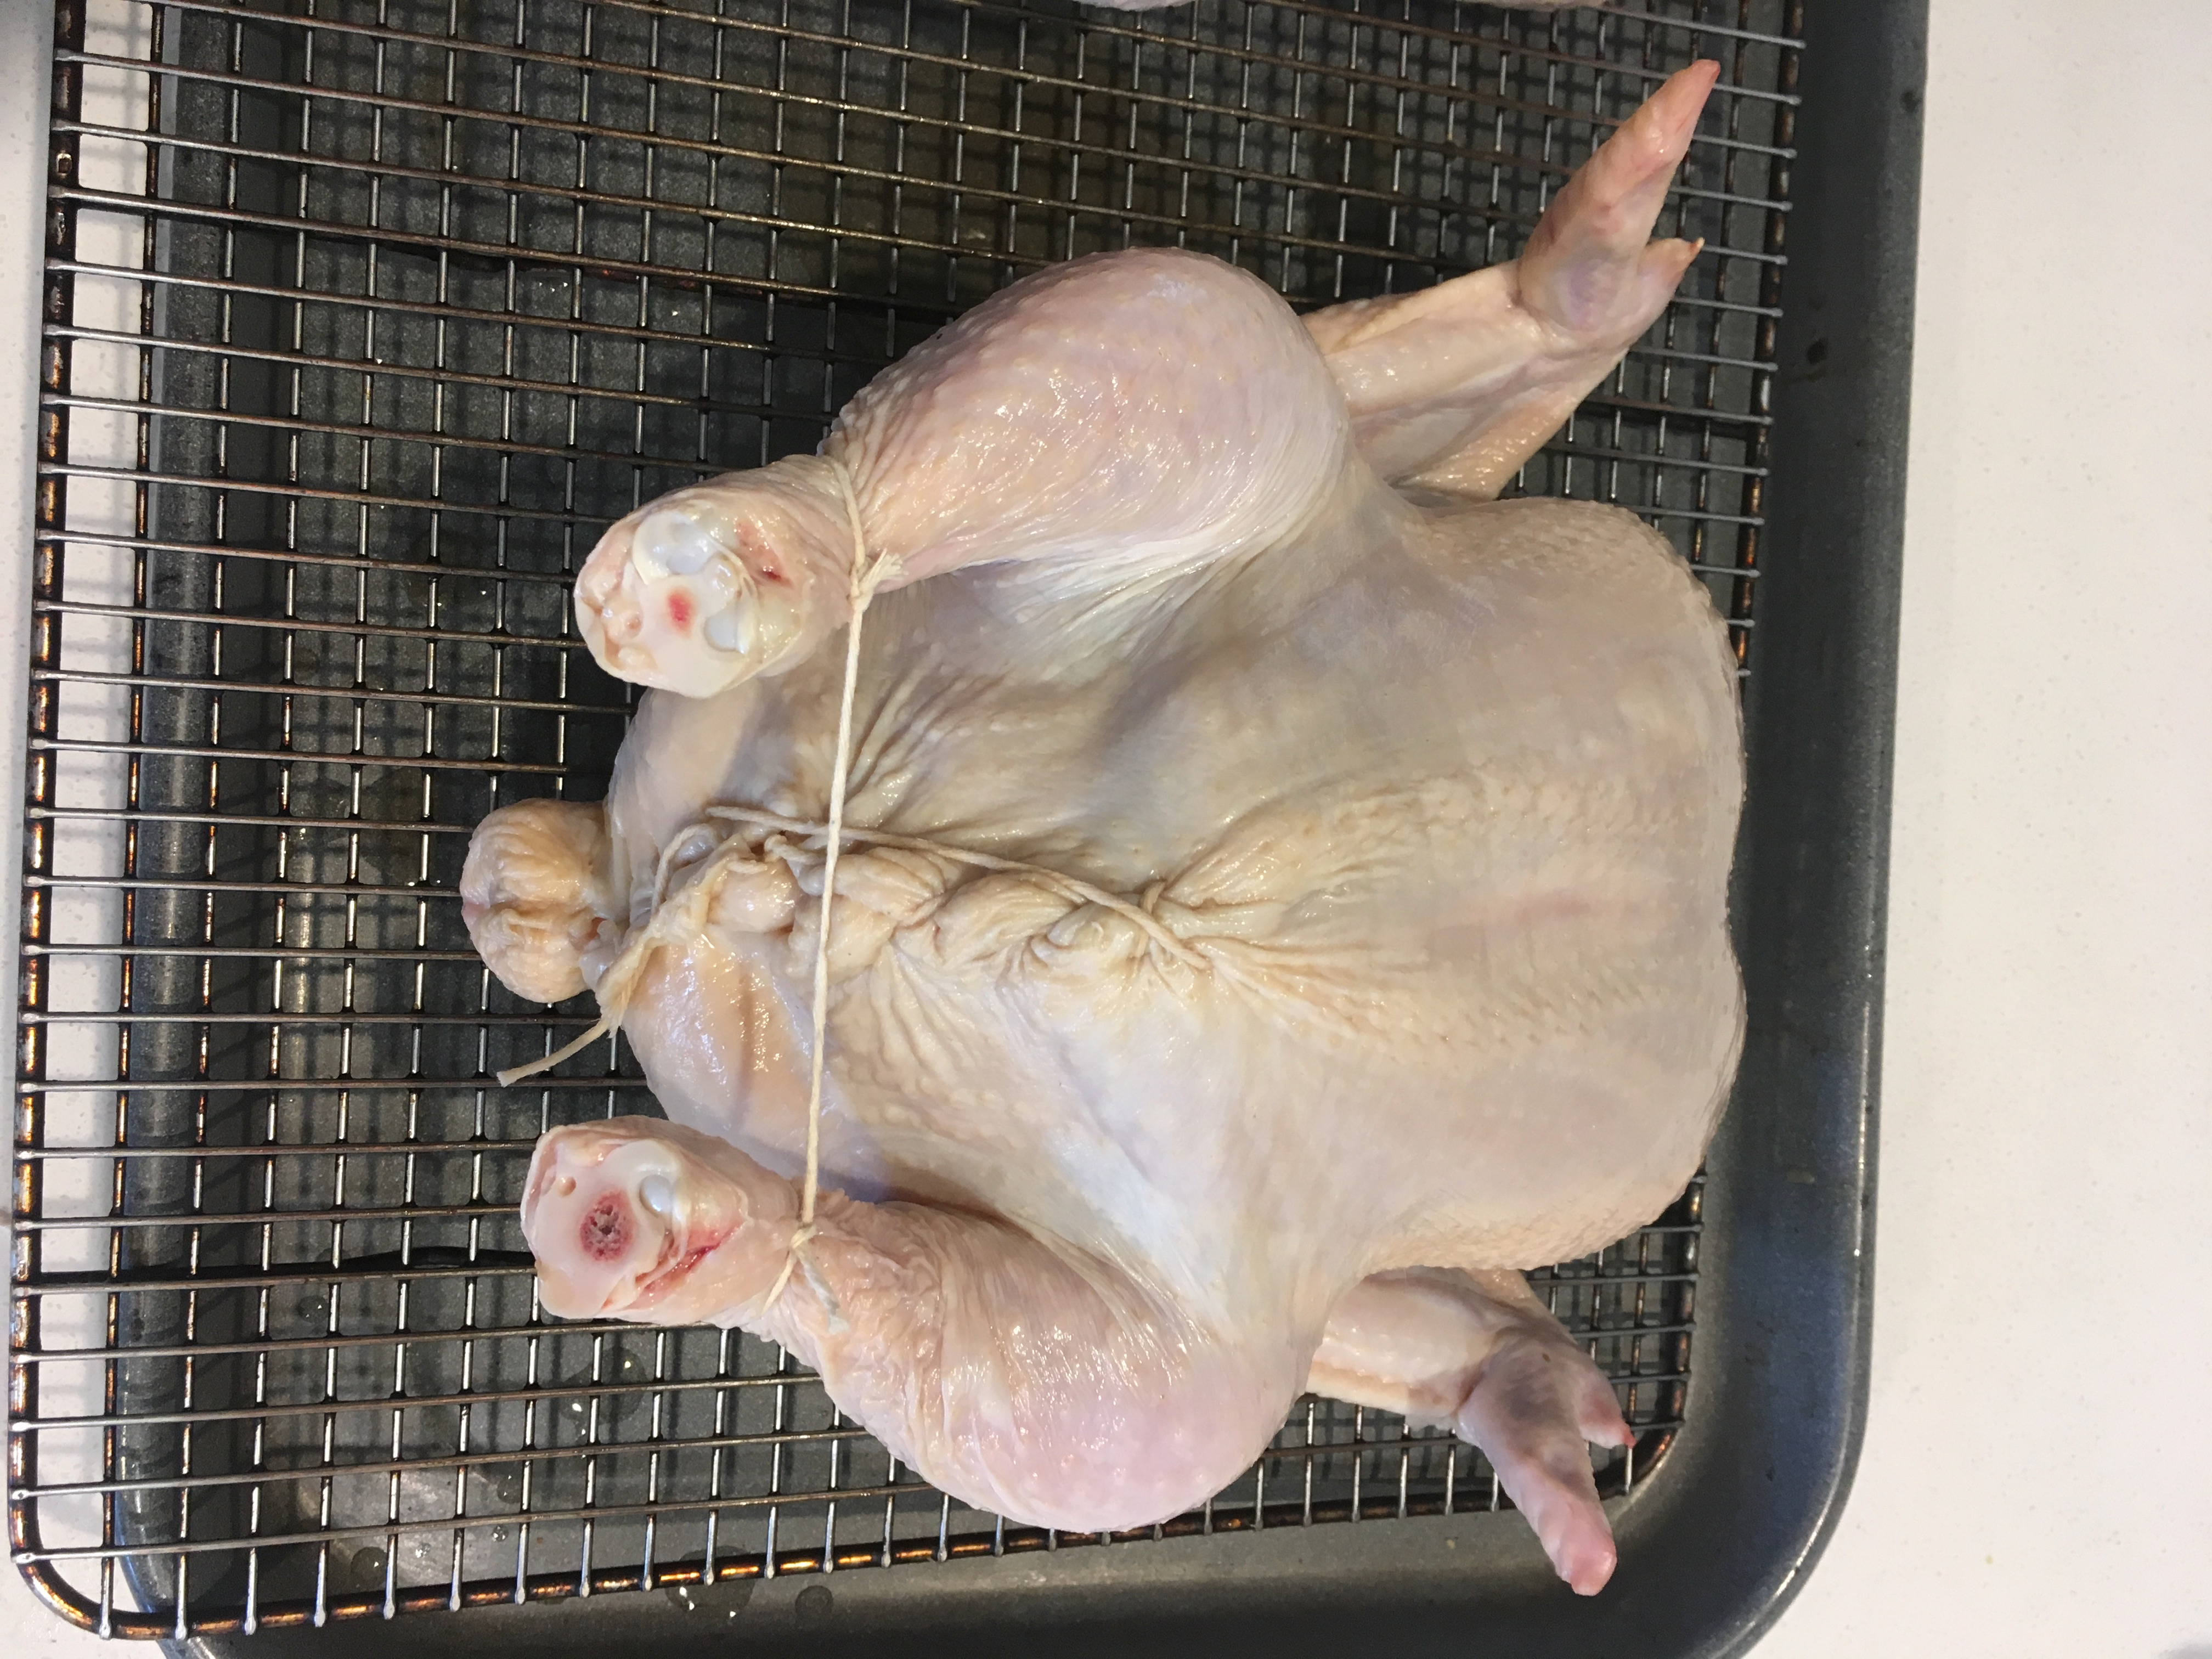
\includegraphics[width=0.25\textwidth]{\imageDir/\fileName/IMG_3219.jpg} \\
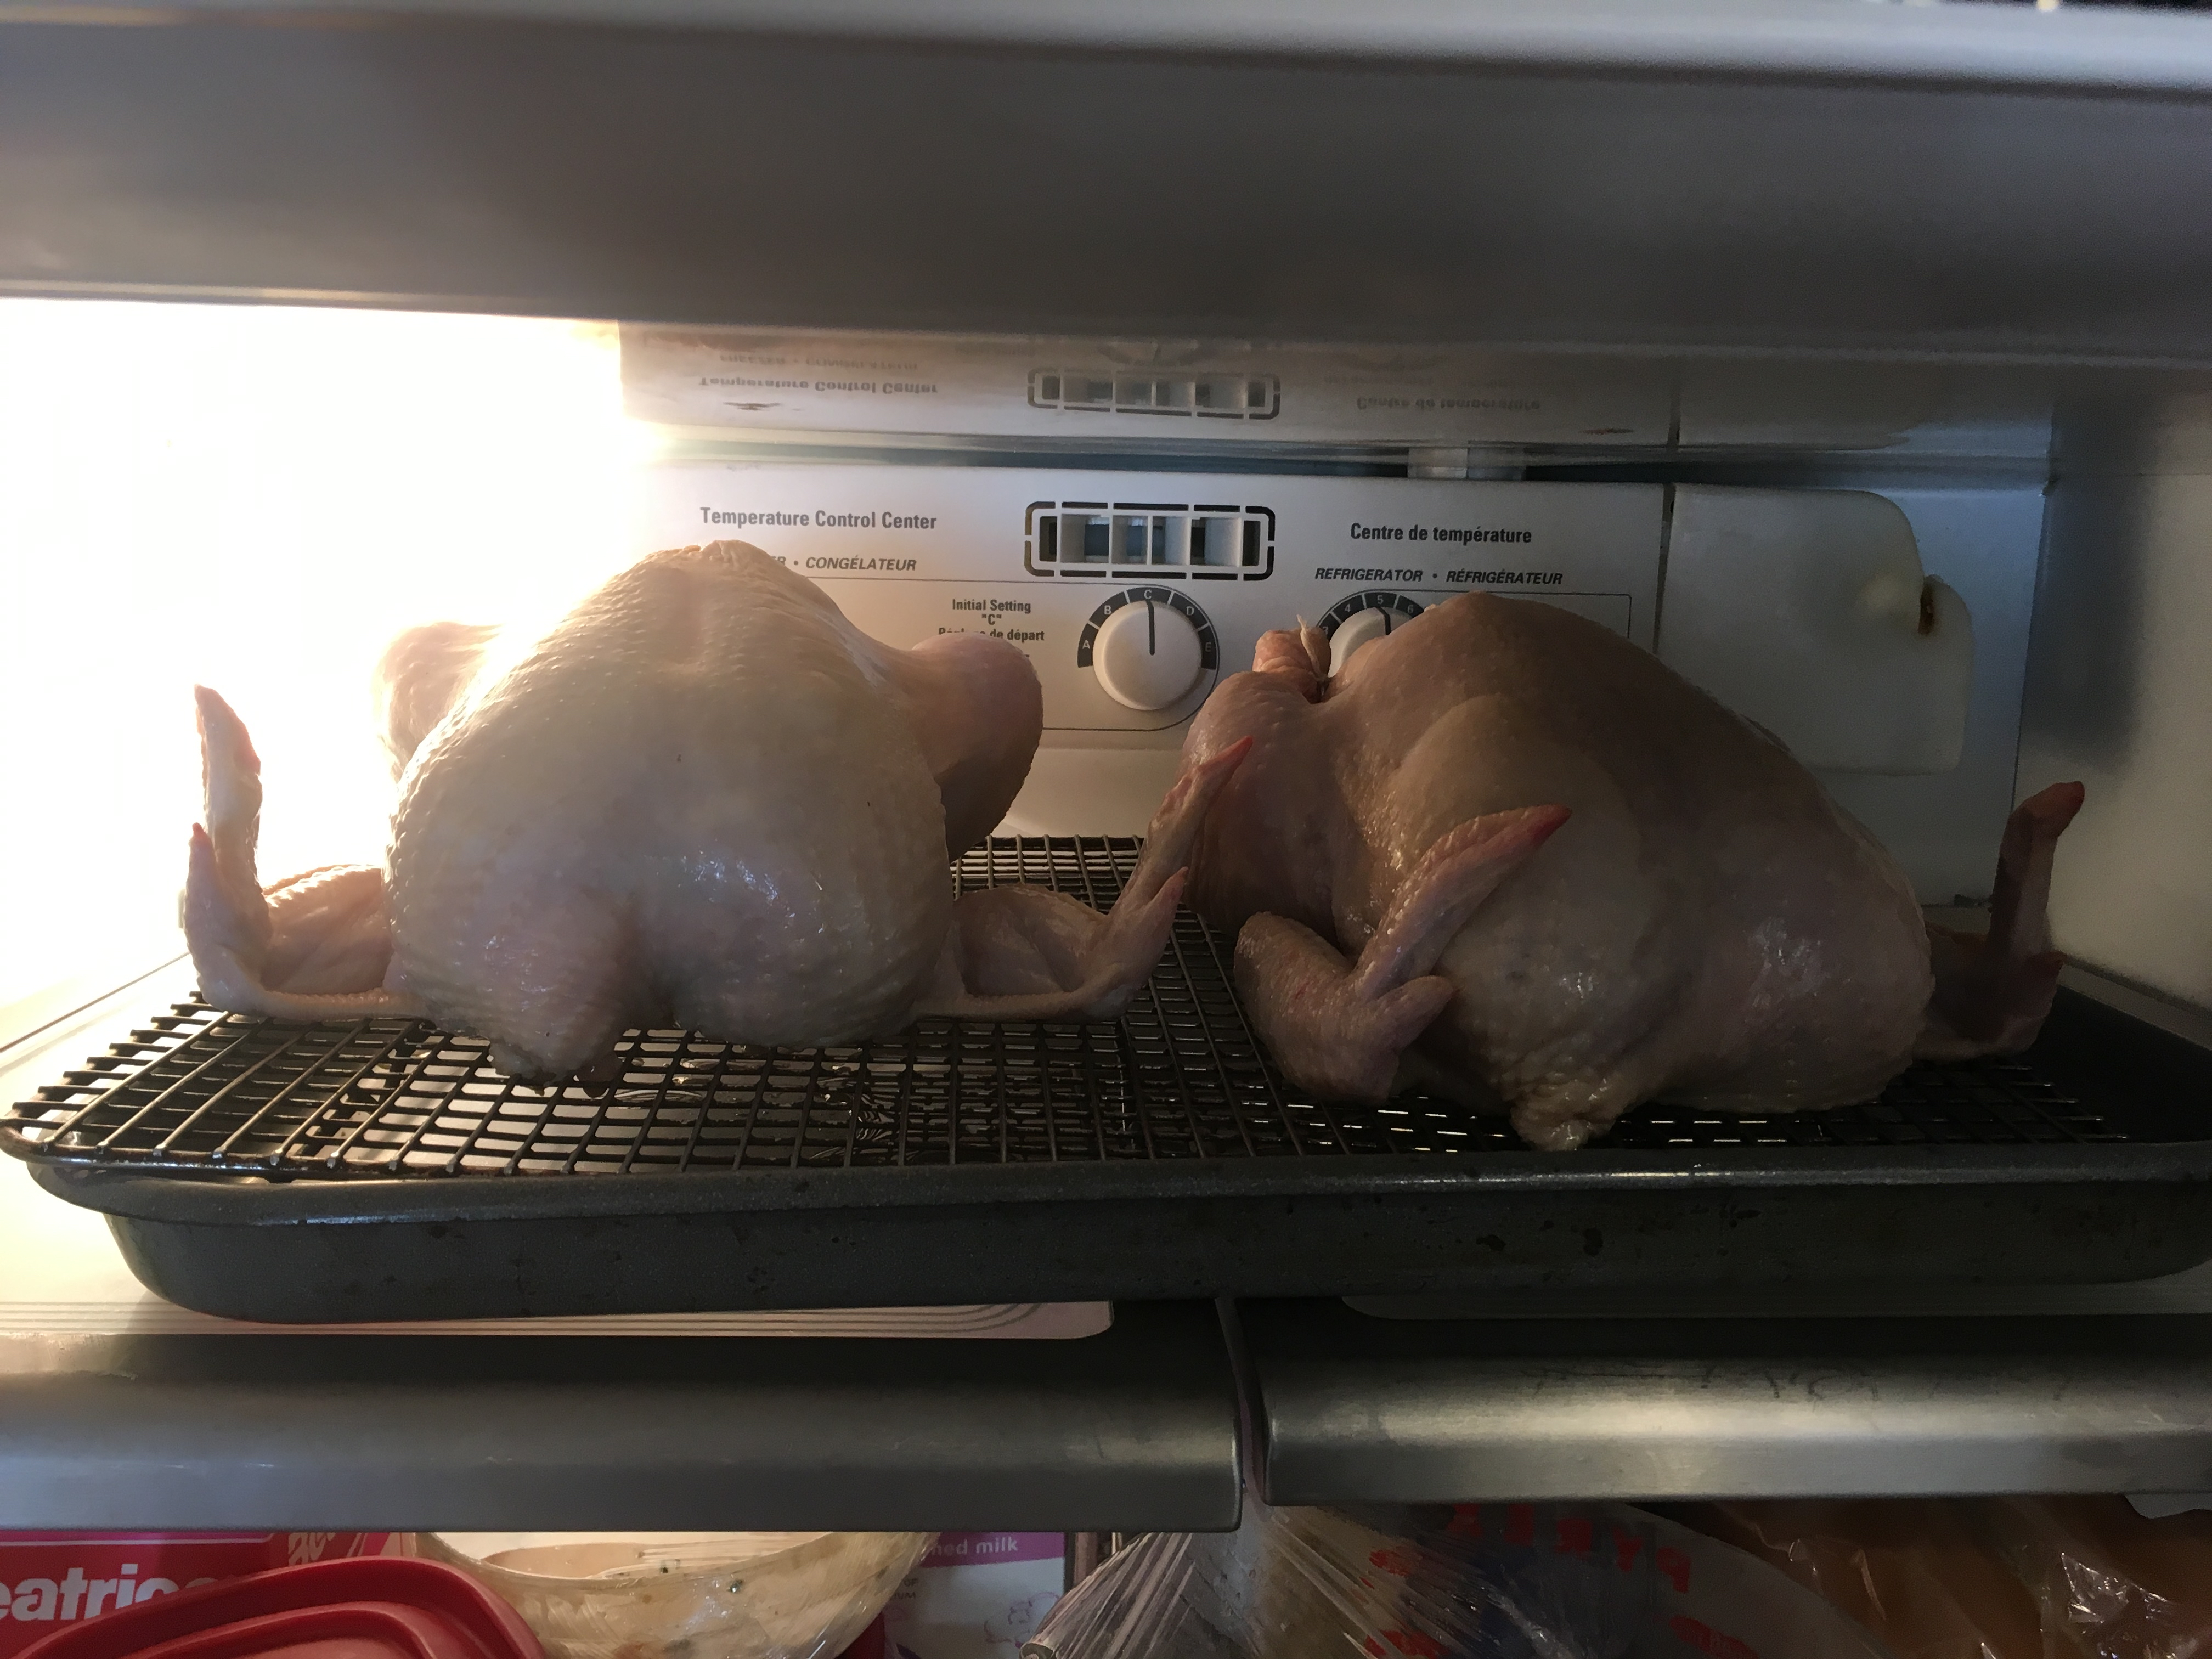
\includegraphics[width=0.25\textwidth]{\imageDir/\fileName/IMG_3220.jpg} &
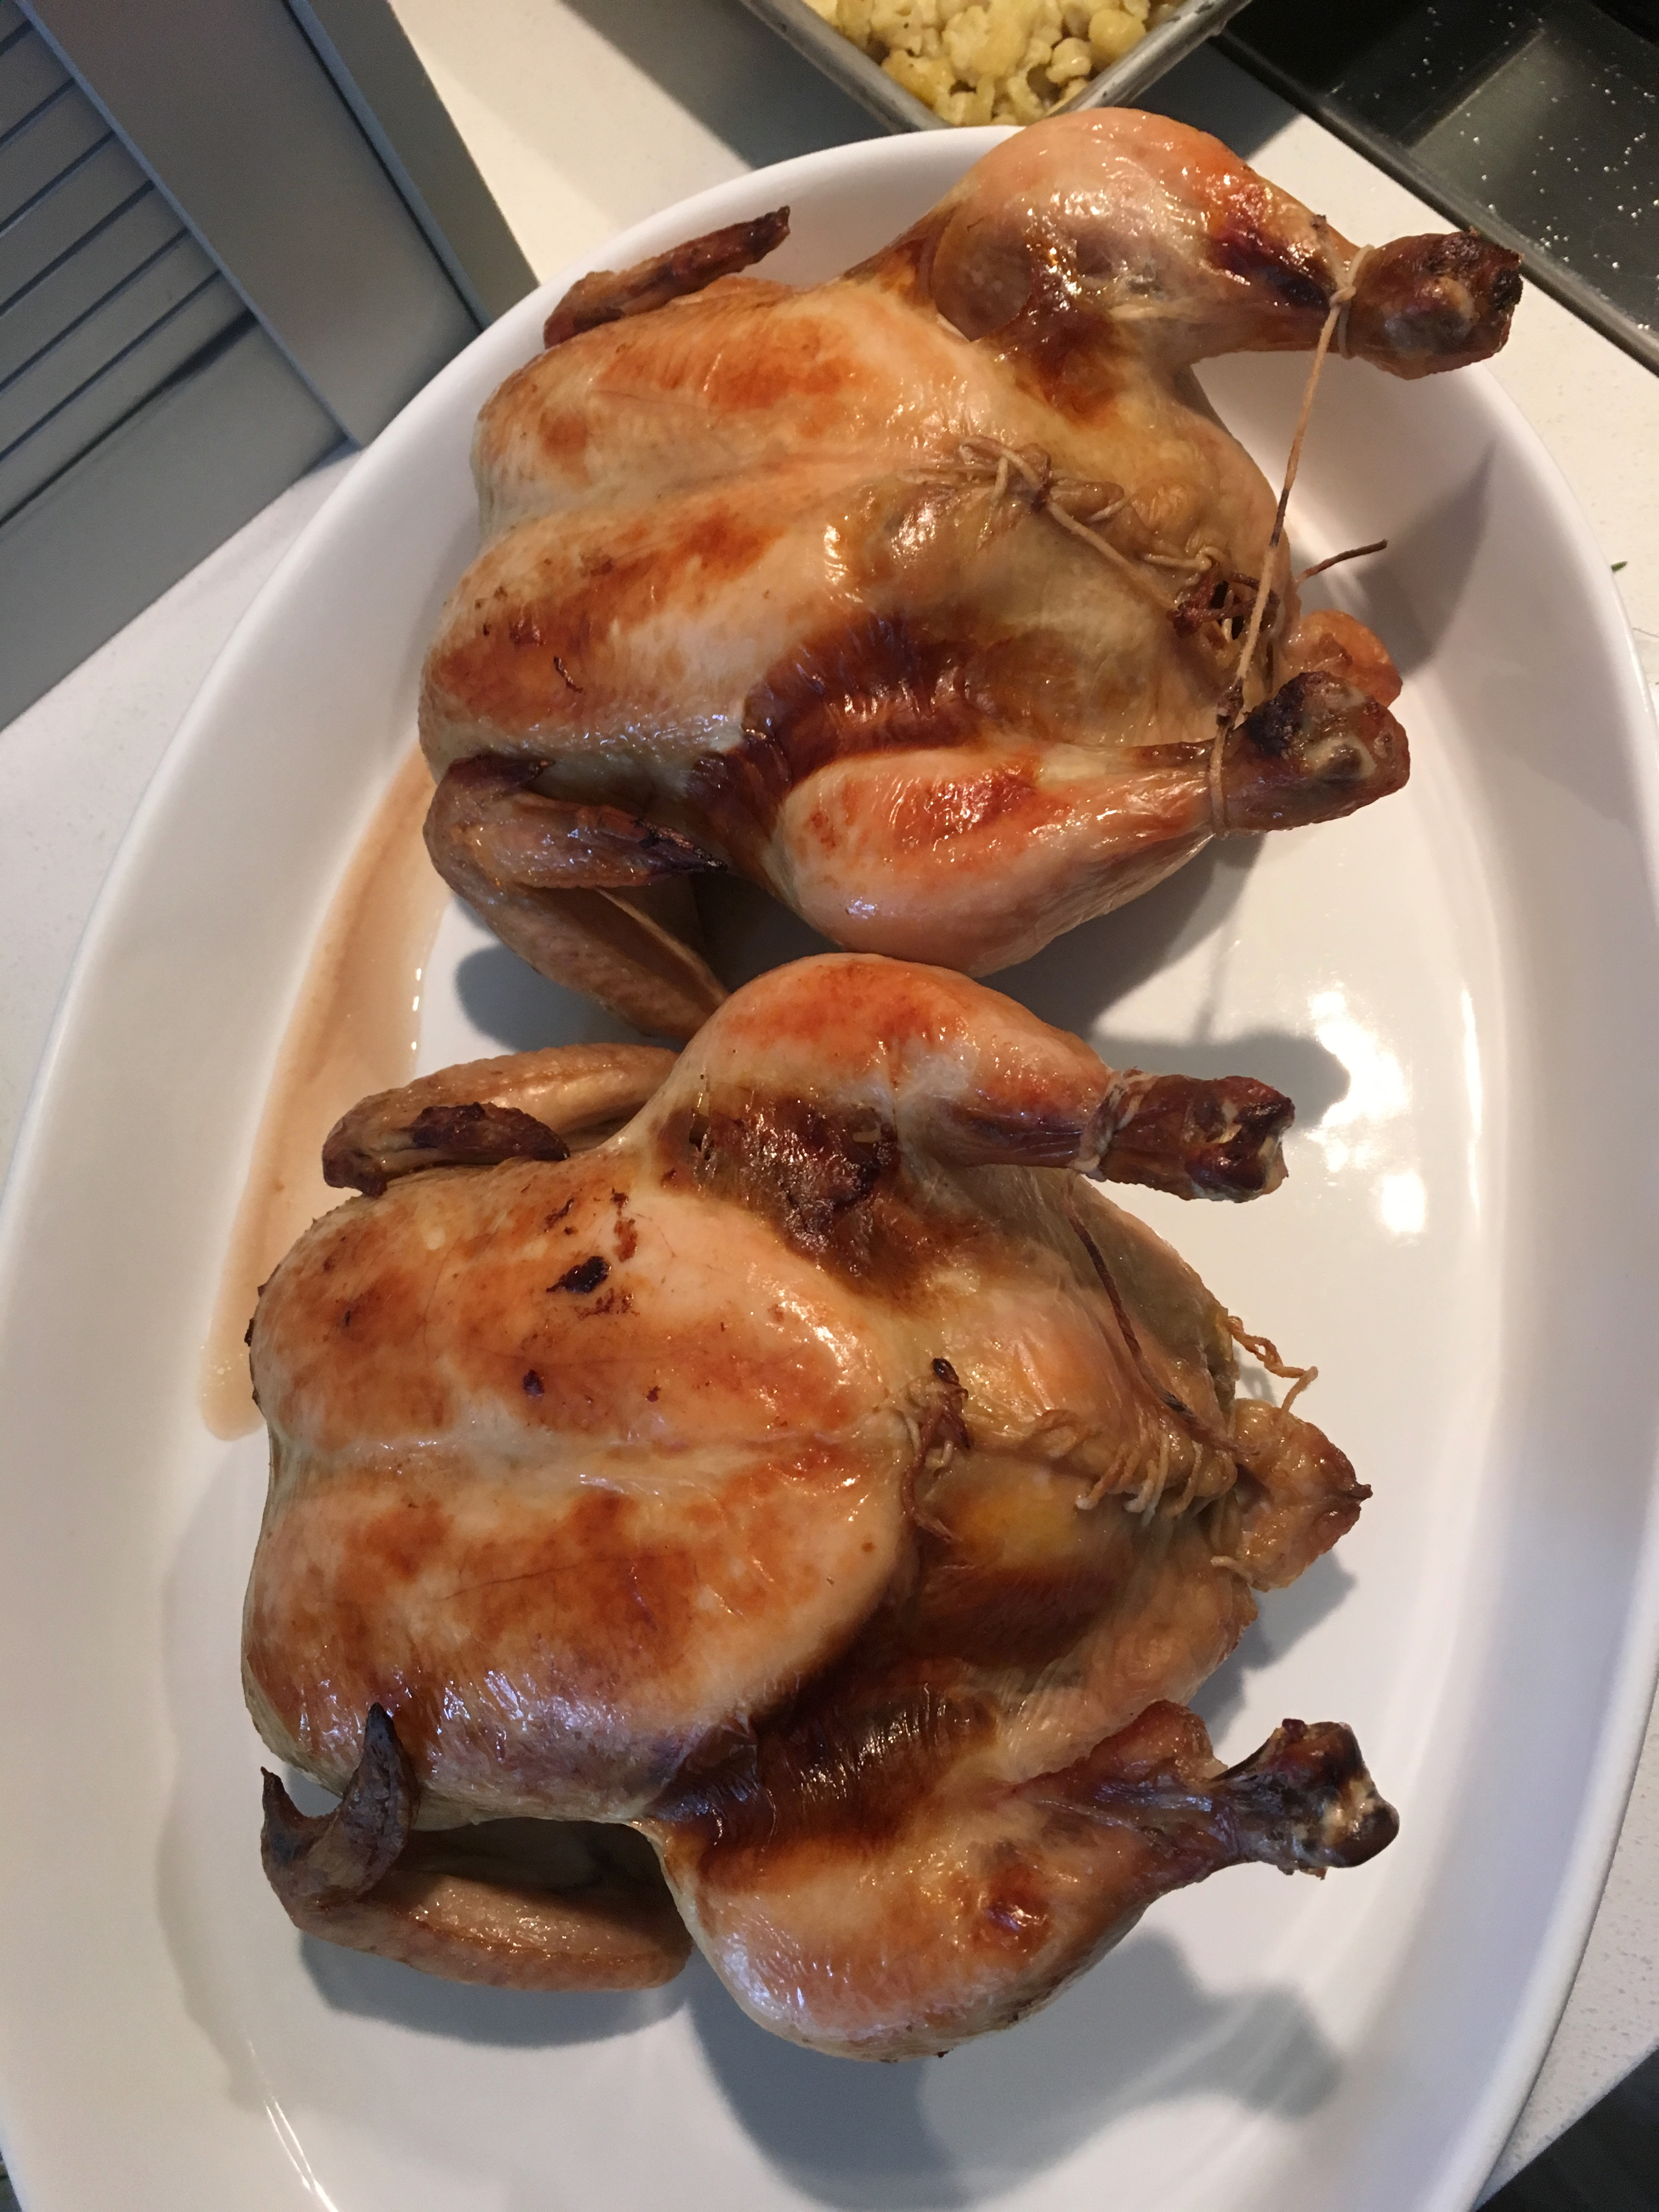
\includegraphics[width=0.25\textwidth]{\imageDir/\fileName/IMG_3228.jpg} \\
\end{tabular}
\end{table}

\end{document}
